% ============================================================================
% Lecture 3: Optimal Carbon Taxation and Deep Uncertainty Quantification
% Design first (constrained optimal taxes and transfers, Kubler/Scheidegger/
% Surbek 2026 JPE:Macro), then quantify (UQ of the SCC, Friedl/Kubler/
% Scheidegger/Usui 2023). Duration: ~90 minutes.
% ============================================================================

\documentclass[aspectratio=169,11pt]{beamer}

% ---------- Theme and colors ----------
\usecolortheme{dove}
\setbeamertemplate{navigation symbols}{}
\setbeamertemplate{footline}{%
  \hfill\usebeamerfont{page number in head/foot}%
  \usebeamercolor[fg]{normal text}%
  \insertframenumber\,/\,\inserttotalframenumber\kern1em\vskip4pt}
\setbeamerfont{frametitle}{size=\huge}

% ---------- Packages ----------
\usepackage[utf8]{inputenc}
\usepackage[T1]{fontenc}
\usepackage{amsmath,amssymb,amsfonts}
\usepackage{bm}
\usepackage{graphicx}
\usepackage{tikz}
\usetikzlibrary{shapes,arrows.meta,positioning,calc,fit,backgrounds,patterns,decorations.pathreplacing}
\usepackage{booktabs}
\usepackage{hyperref}
\usepackage{multicol}
\usepackage{xcolor}
\usepackage{natbib}
\usepackage{makecell}
\usepackage{tabularx}
\usepackage[font=footnotesize,labelfont=bf]{caption}
\usepackage[font=footnotesize,labelfont=bf]{subcaption}

\graphicspath{{fig/}}

% ---------- Custom colors ----------
\definecolor{uzhblue}{rgb}{0,0,0.5}
\definecolor{uzhgreylight}{RGB}{236,238,241}
\definecolor{uzhgreydark}{RGB}{81,86,94}
\definecolor{harvardcrimson}{RGB}{153,0,0}
\definecolor{unil@blue}{RGB}{0,140,204}
\definecolor{unil@black}{RGB}{35,31,32}
\definecolor{darkgreen}{RGB}{0,100,0}
\definecolor{darkred}{RGB}{139,0,0}
\definecolor{softblue}{RGB}{70,130,180}
\definecolor{softorange}{RGB}{230,159,0}
\definecolor{softgreen}{RGB}{0,158,115}

% ---------- Set beamer colors ----------
\setbeamercolor{frametitle}{bg=uzhgreylight, fg=uzhblue}
\setbeamercolor{title}{fg=uzhblue}
\setbeamercolor{structure}{fg=uzhblue}
\setbeamercolor{block title}{bg=unil@blue, fg=white}
\setbeamercolor{block body}{bg=uzhgreylight}
\setbeamercolor{block title alerted}{bg=darkred,fg=white}
\setbeamercolor{block body alerted}{bg=red!5}
\setbeamercolor{block title example}{bg=darkgreen,fg=white}
\setbeamercolor{block body example}{bg=green!5}
\setbeamercolor{item}{fg=unil@black}
\setbeamercolor{normal text}{fg=unil@black}

% ---------- Emphasis and hyperlinks ----------
\newcommand{\emphc}[1]{\textcolor{harvardcrimson}{#1}}
\newcommand{\key}[1]{\textbf{\textcolor{uzhblue}{#1}}}
\newcommand{\keyc}[1]{\textcolor{uzhblue}{#1}}
\newcommand{\stoch}[1]{\textcolor{darkred}{#1}}
\hypersetup{colorlinks,linkcolor=harvardcrimson,urlcolor=harvardcrimson}

% ---------- Math commands ----------
\newcommand{\R}{\mathbb{R}}
\newcommand{\E}[1]{\mathbb{E}\!\left[#1\right]}
\DeclareMathOperator*{\argmin}{arg\,min}
\DeclareMathOperator*{\argmax}{arg\,max}

% ---------- Appendix frame numbering ----------
\usepackage{appendixnumberbeamer}

% ---------- Title ----------
\title[CEMRACS 2026 $\cdot$ Optimal Taxation \& Deep UQ]
{Computational and AI Methods in Climate Economics}
\subtitle{Lecture 3 --- Optimal carbon taxation and deep uncertainty quantification: solve once, ask many questions}
\author{Simon Scheidegger}
\institute[HEC Lausanne]{HEC Lausanne $\cdot$ Grantham Research Institute, LSE}
\date{July 15, 2026 \,$\cdot$\, CIRM, Marseille, France}

\begin{document}


% ============================================================================
% PART 0: TITLE & OUTLINE
% ============================================================================

% --- Slide 1: Title ---
{\setbeamercolor{background canvas}{bg=uzhgreylight}
\begin{frame}
\titlepage
\vspace{-0.75cm}
\begin{center}
{\scriptsize Based on: K\"ubler, Scheidegger \& Surbek (2026), ``Using Machine Learning to Compute Constrained Optimal Carbon\\
Tax Rules,'' \emph{Journal of Political Economy: Macroeconomics}, and Friedl, K\"ubler, Scheidegger \& Usui (2023),\\
``Deep Uncertainty Quantification.''}\\[3pt]
{\scriptsize Replication code: \url{https://github.com/sischei/JPE_Macro_Using_ML_to_compute_constrained_optimal_carbon_tax_rules}}\\[2pt]
{\scriptsize Materials: \url{https://github.com/sischei/cemracs2026_DEQN}}
\end{center}
\end{frame}
}

% --- Slide 2: Roadmap ---
\begin{frame}{Roadmap of This Lecture}
\vspace{0.2em}
\begin{columns}[T]
\column{0.48\textwidth}
\textbf{Part A}
\begin{itemize}
    \item \textbf{Part I.} Motivation: from solving models (Lectures 1--2) to answering policy questions --- three operators on one surrogate
    \item \textbf{Part II.} The two-surrogate pipeline, generalized: pseudo-states, quantities of interest, post-processing operators
    \item \textbf{Part III.} \emphc{Design}: constrained optimal carbon taxes and transfers in a stochastic OLG IAM --- three policy scenarios, from unconstrained to Pareto-improving
\end{itemize}

\column{0.48\textwidth}
\textbf{Part B}
\begin{itemize}
    \item \textbf{Part IV.} \emphc{Quantify}: deep uncertainty quantification of the social cost of carbon --- univariate effects, Sobol' indices, Shapley values
    \item \textbf{Part V.} Synthesis: one surrogate, three questions; practical guidance; extensions and open questions
\end{itemize}
\end{columns}
\end{frame}

% --- Slide 3: Learning objectives ---
\begin{frame}{Learning objectives}
\textbf{By the end of this lecture you should be able to:}
\begin{itemize}
  \item Extend pseudo-state surrogates from estimation to policy design and uncertainty quantification
  \item Solve constrained policy problems, including Pareto constraints, directly on the surrogate
  \item Add a Gaussian process and Bayesian-active-learning layer when each QoI evaluation needs heavy Monte Carlo
  \item Compute the social cost of carbon and welfare quantities of interest from surrogate simulations
  \item Rank parameter uncertainties via univariate effects, Sobol' indices, and Shapley values
\end{itemize}
\end{frame}


% ============================================================================
% PART I: MOTIVATION --- FROM SOLVING TO ASKING QUESTIONS
% ============================================================================

% --- Section divider ---
\begin{frame}{}
\vfill
\begin{center}
{\Huge \textcolor{uzhblue}{\textbf{Part I}}}\\[12pt]
{\LARGE From Solving Models to Answering Policy Questions}
\end{center}
\vfill
\end{frame}

% --- Where Lectures 1 and 2 left us ---
\begin{frame}{Where Lectures 1 and 2 Left Us}
\footnotesize
\begin{columns}[c]
\begin{column}{0.62\textwidth}
\textbf{The stack so far:}
\begin{itemize}\itemsep1pt
  \item \textbf{Lecture 1:} Deep Equilibrium Nets solve dynamic stochastic models globally by minimizing equilibrium residuals along simulated paths.
  \item \textbf{Lecture 2 (Part 1):} the DICE/CDICE climate--economy model, solved globally with DEQNs.
  \item \textbf{Lecture 2 (Part 2):} surrogates with parameters as \emph{pseudo-states} decouple solving from asking; GP regression and Bayesian active learning make expensive maps cheap; SMM estimation rode on top.
\end{itemize}
\vspace{0.15em}
\textbf{The pivot:} estimation treats $\bm{\theta}$ as unknown but \emphc{fixed}. Two questions remain:
\begin{itemize}\itemsep1pt
  \item What if some inputs are not parameters at all, but \emphc{choices}?
  \item What if $\bm{\theta}$ \emphc{stays uncertain} after all we know?
\end{itemize}
\vspace{0.15em}
Today's mantra: \emphc{solve once, ask many questions.}
\end{column}
\begin{column}{0.36\textwidth}
\centering
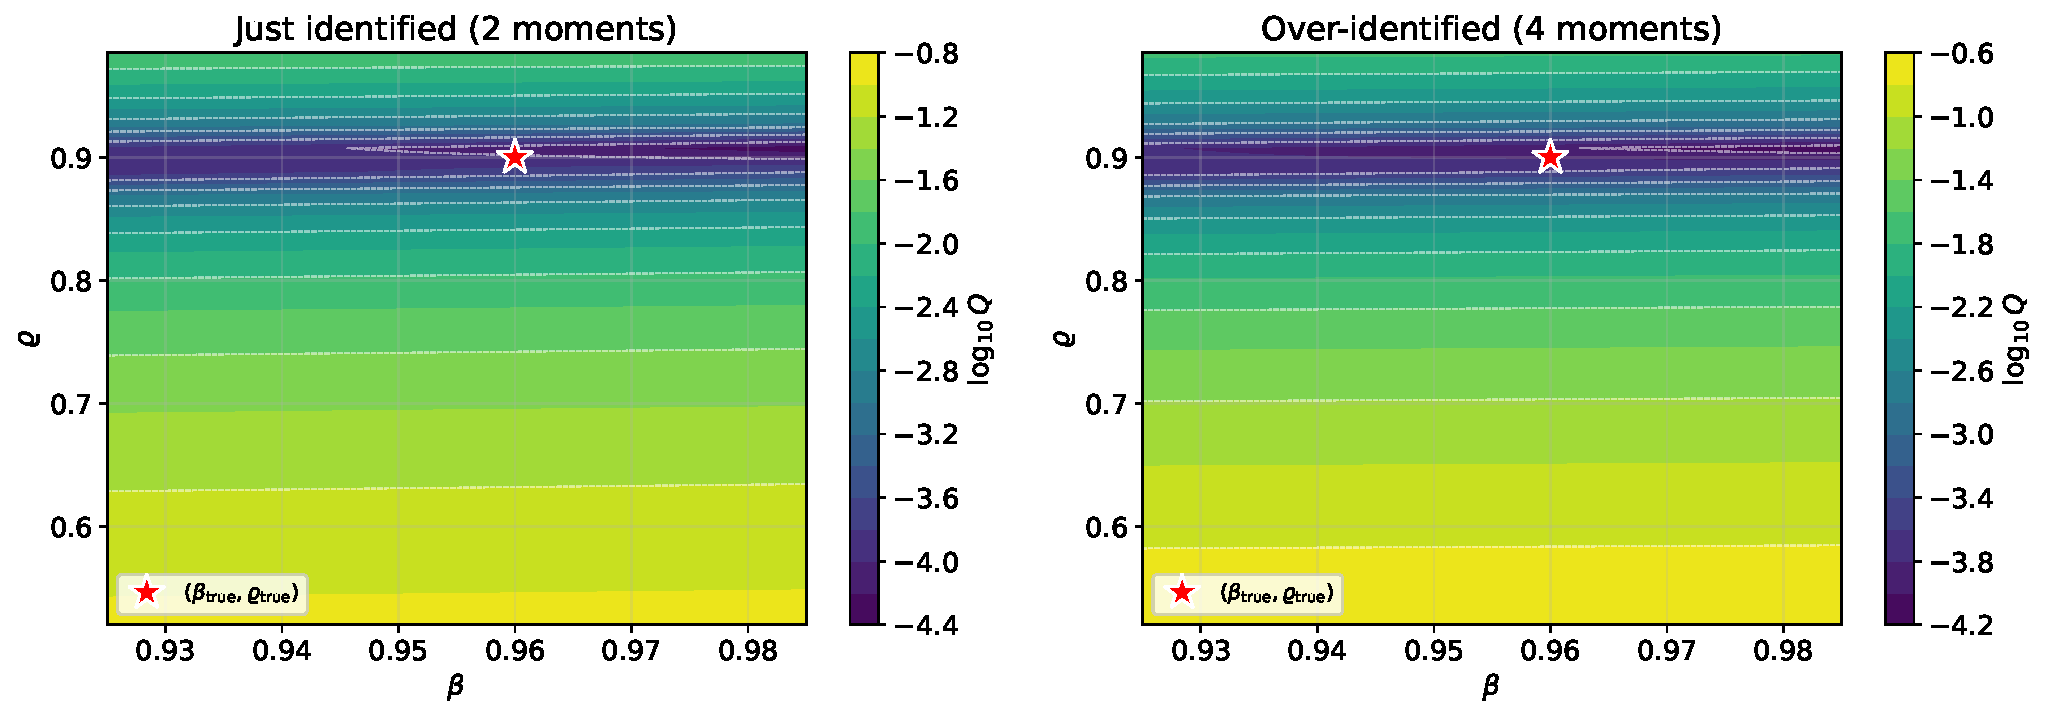
\includegraphics[width=\linewidth]{l15/joint_criterion_contour.pdf}
{\scriptsize Lecture 2's estimation surrogate: the criterion's shape, not just its argmin, carried the lesson.}
\end{column}
\end{columns}
\end{frame}

% --- Three operators, one surrogate ---
\begin{frame}{Three Operators, One Surrogate}
\small
Three questions ride on one parametric surrogate. Lecture 2 asked the first; today we work out \emphc{design} (Part III) and \emphc{quantify} (Part IV) in full.
\vspace{0.5em}
\begin{center}
\footnotesize
\begin{tabular}{p{0.09\textwidth}p{0.23\textwidth}p{0.36\textwidth}p{0.17\textwidth}}
\toprule
\textbf{Operator} & \textbf{Question} & \textbf{Post-processing} & \textbf{Where} \\
\midrule
\emphc{Estimate} & Which parameters fit the data? & $\argmin$ of an SMM criterion over $\bm{\theta}$ & Lecture 2 (Part 2) \\[3pt]
\emphc{Design} & Which policy is best? & constrained $\argmax$ of a welfare QoI over $\vartheta$ & Part III (carbon taxes) \\[3pt]
\emphc{Quantify} & Which parameter uncertainties matter? & propagate $p(\bm{\theta})$ through a QoI: univariate effects, Sobol' indices, Shapley values & Part IV (SCC: social cost of carbon) \\
\bottomrule
\end{tabular}
\end{center}
\vspace{0.5em}
Identical machinery throughout: the \emphc{two-surrogate pipeline}. Surrogate 1 solves the equilibrium over states and pseudo-states; Surrogate 2 maps parameters to quantities of interest. Only the post-processing operator changes.
\end{frame}

% --- The challenge: climate risk & heterogeneity ---
\begin{frame}{The Challenge: Climate Risk \& Heterogeneity}
    \begin{columns}[c]
        \begin{column}{0.45\textwidth}
            \centering
            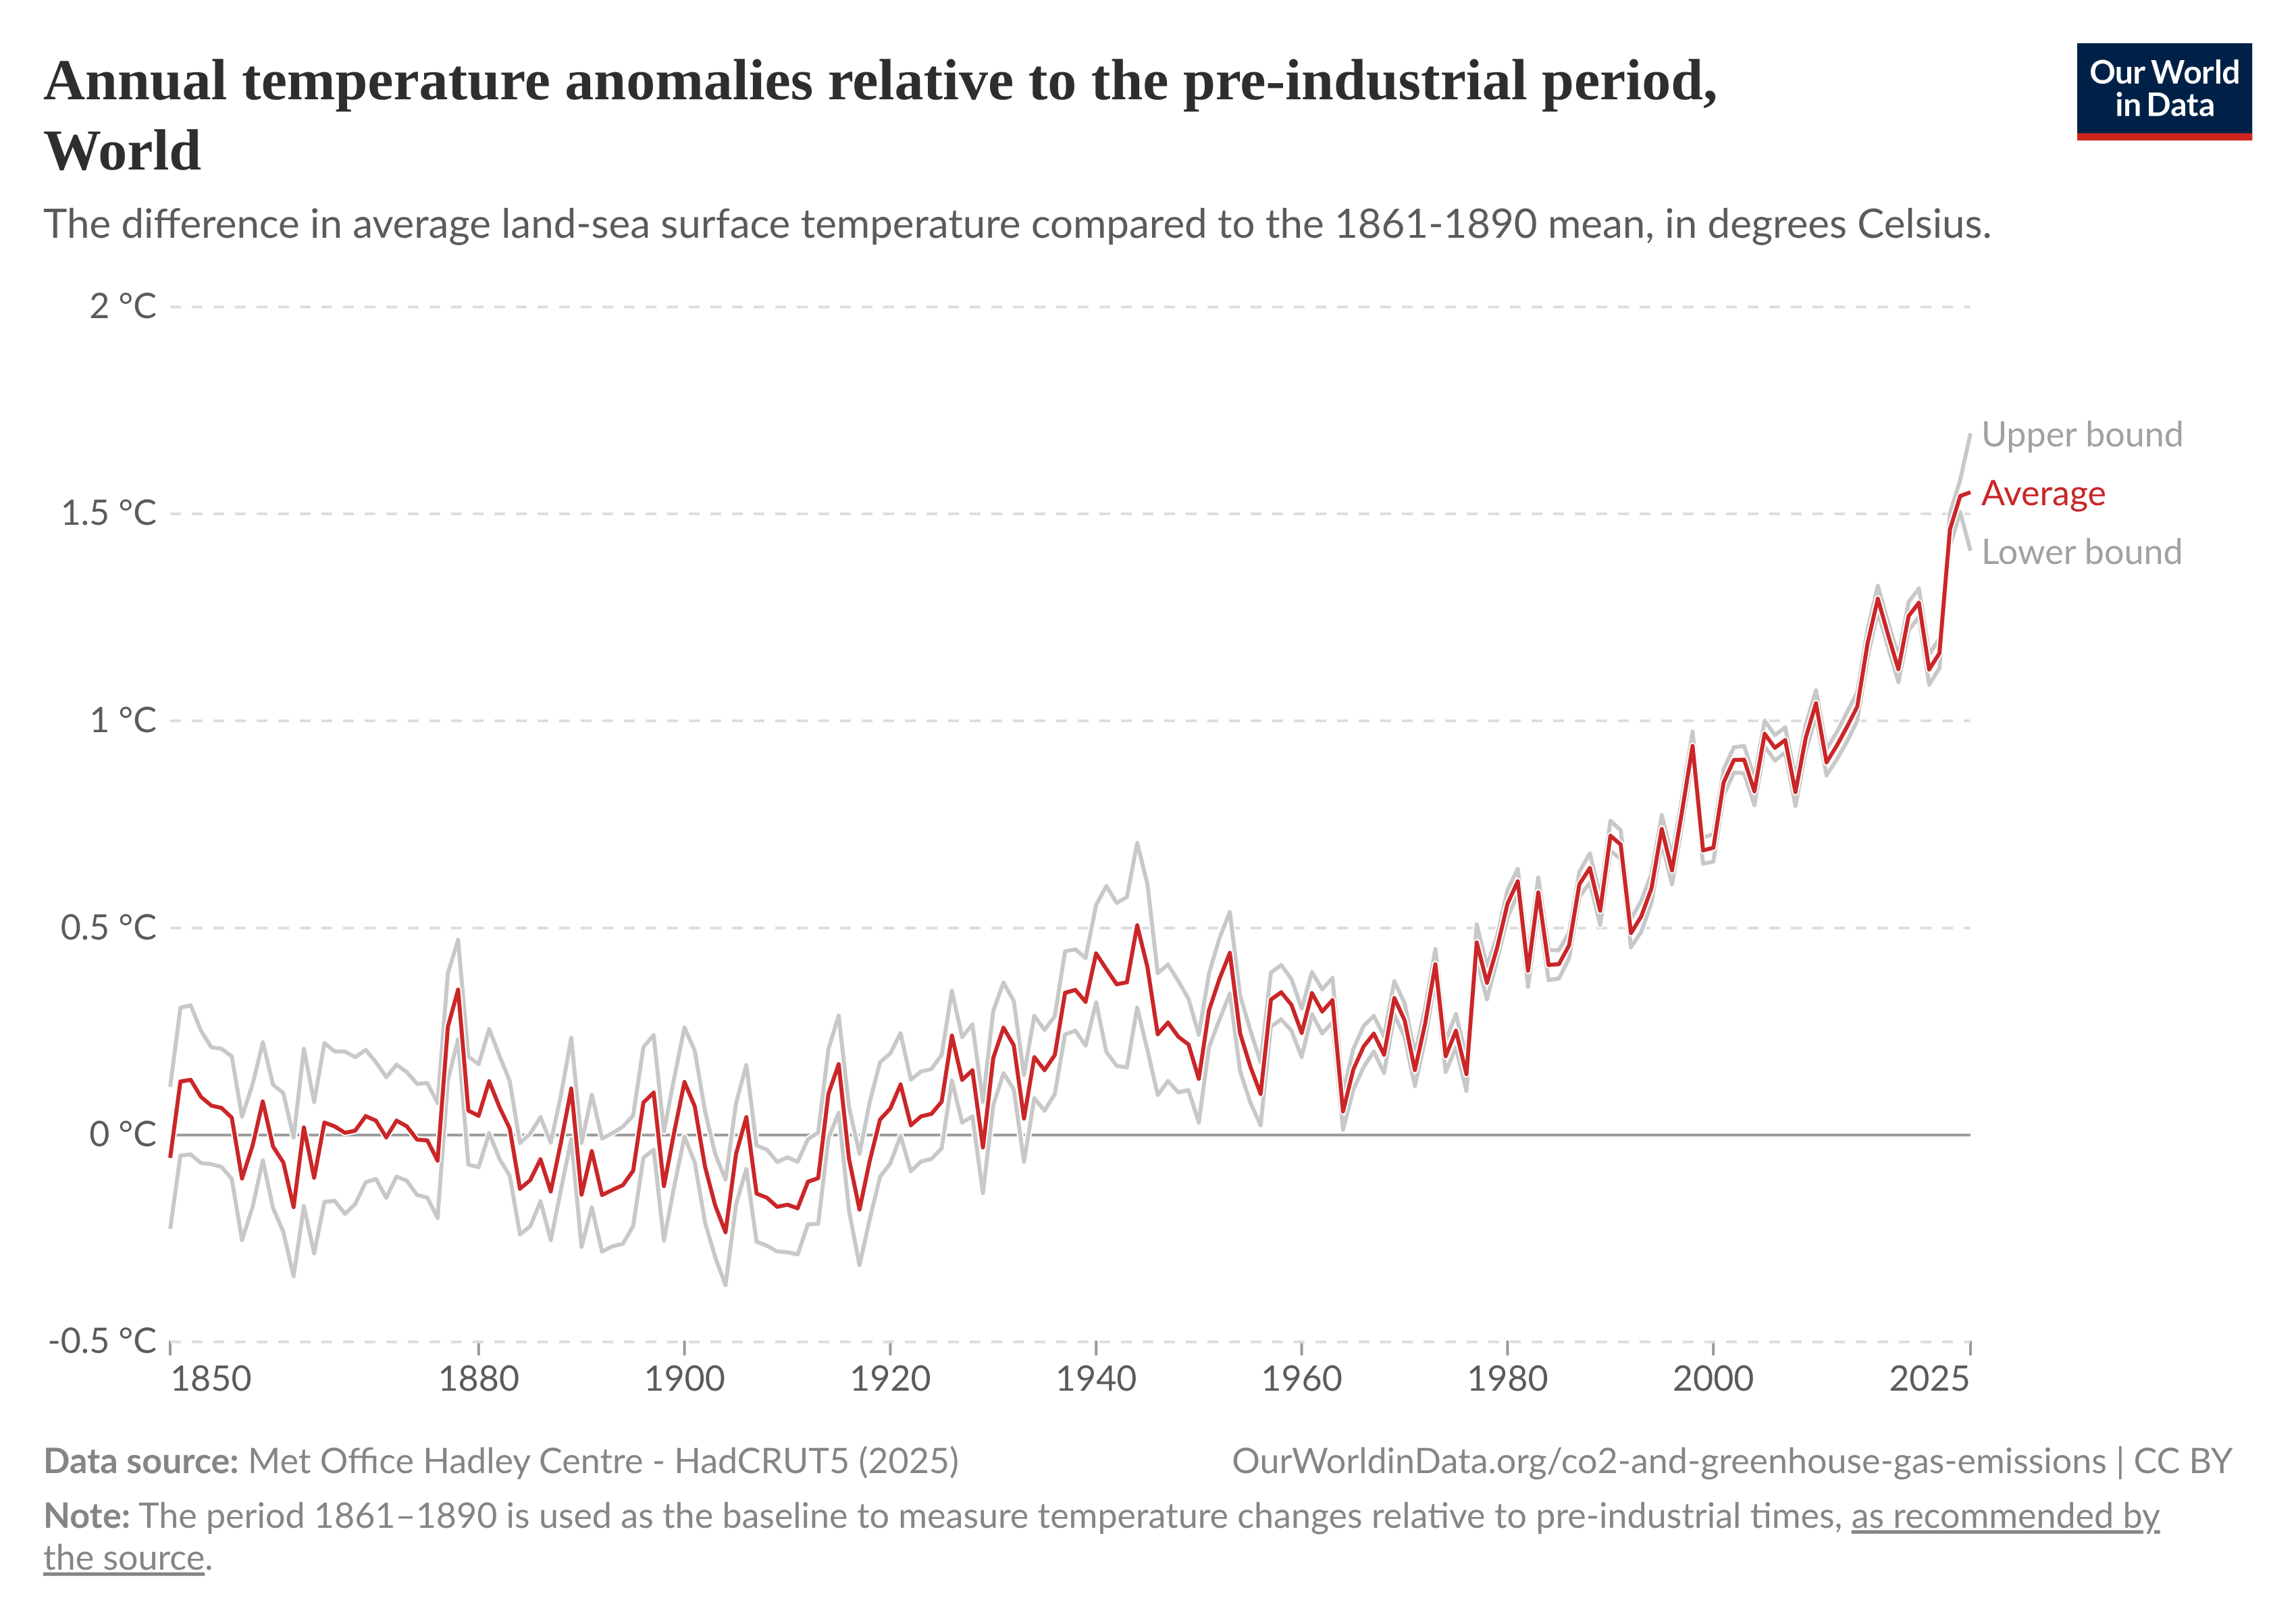
\includegraphics[width=0.85\linewidth]{tax/temperature-anomaly.png}

            \vspace{0.4em}

            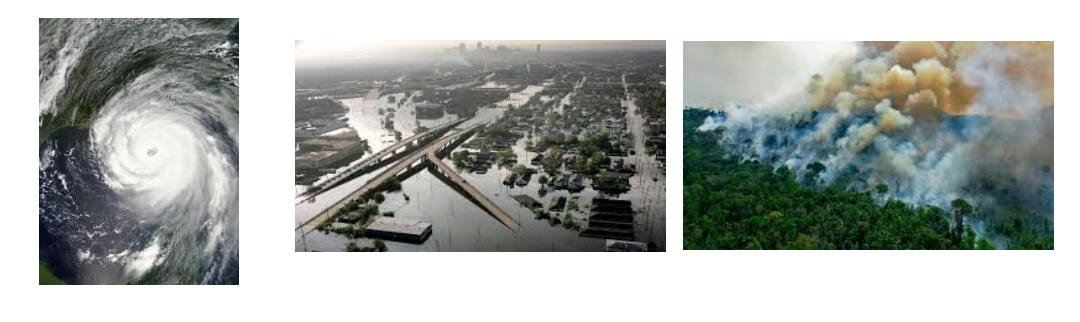
\includegraphics[width=0.85\linewidth]{tax/global-warming.png}
        \end{column}
        \begin{column}{0.55\textwidth}
            \small
            \begin{itemize}
                \setlength\itemsep{0.8em}
                \item \textbf{Systemic Risk:} Climate change poses a fundamental threat to global economic stability and human welfare.
                \item \textbf{Non-Linear Dynamics:} Tipping points introduce the risk of irreversible, catastrophic environmental shifts.
                \item \textbf{Distributional Impact:} Effects will be highly heterogeneous, creating profound equity challenges across regions and generations.
                \item \textbf{Literature Context:} These macro-financial linkages are detailed in the recent review Fernandez-Villaverde, Gillingham, and Scheidegger (2025).
            \end{itemize}
        \end{column}
    \end{columns}
\end{frame}

% --- Two policy questions, one computational wall ---
\begin{frame}{Two Policy Questions, One Computational Wall}
\footnotesize
\begin{columns}[t]
\begin{column}{0.48\textwidth}
\textbf{Design: which carbon tax is best?} {\tiny (Part III)}
\begin{itemize}\itemsep1pt
  \item \textbf{The Consensus:} Carbon pricing is widely regarded as the most efficient tool to mitigate emissions.
  \item \textbf{The Difficulty:} With heterogeneous agents (e.g., OLG), simple taxes create winners and losers, threatening political feasibility.
  \item \textbf{The Objective:} A systematic way to compute \keyc{constrained optimal taxes} under stochastic risks (tipping points) and political constraints (Pareto improvements): most work relies on \keyc{simplifying assumptions} or heuristic ``guessing''.
\end{itemize}
\end{column}
\begin{column}{0.48\textwidth}
\textbf{Quantify: how uncertain is the SCC?} {\tiny (Part IV)}
\begin{itemize}\itemsep1pt
  \item \key{Carbon taxation}: widely supported policy response to the climate change problem.
  \item The tax level is based on the social cost of carbon (SCC): the marginal loss caused by an extra ton of CO$_2$ emissions.
  \item SCC values are computed with \key{integrated assessment models} (IAMs; Lecture 2, Part 1).
  \item IAMs are subject to \key{significant parametric uncertainty, model uncertainty, and climate risks of tipping points}.
\end{itemize}
\end{column}
\end{columns}
\vspace{0.4em}
{\scriptsize \emphc{The wall:} both questions need thousands of model evaluations. IAMs are complex non-linear models highly susceptible to the curse of dimensionality; evaluating expected welfare requires 10{,}000 Monte Carlo paths per policy $\vartheta$. Lecture 2's answer carries over: with a deep surrogate, the inner loop is three orders of magnitude cheaper.}
\end{frame}


% ============================================================================
% PART II: THE TWO-SURROGATE PIPELINE, GENERALIZED
% ============================================================================

% --- Section divider ---
\begin{frame}{}
\vfill
\begin{center}
{\Huge \textcolor{uzhblue}{\textbf{Part II}}}\\[12pt]
{\LARGE The Two-Surrogate Pipeline, Generalized}
\end{center}
\vfill
\end{frame}

% --- Pipeline in a nutshell ---
\begin{frame}{The Two-Surrogate Pipeline in a Nutshell}
\small
  \begin{itemize}
    \item \textbf{Step 1: Global solution with DEQN (Surrogate 1)}
      \begin{itemize}
        \item \keyc{Solve the model as a function of states and pseudo-states in one go}: train on $\tilde{x} = (x, \bm{\theta}, \vartheta)$, exactly the pseudo-state trick of Lecture 2.
        \item \keyc{For linear tax rules in cumulative emissions, $\kappa$, $TP$}: 4 tax pseudo-states $\vartheta = (\vartheta_0, \vartheta_E, \vartheta_\kappa , \vartheta_{TP})$, plus \keyc{12 from transfer shares}.
      \end{itemize}
      $\Rightarrow$ \keyc{Once trained, the solution allows us to simulate data essentially for free}.
    \item \textbf{Step 2: Simulate quantities of interest (Surrogate 2 where needed)}
      \begin{itemize}
        \item $\widehat{\mathrm{QoI}}(\cdot)$ generalizes Lecture 2's moment map $m(\theta)$: there a handful of moments; in Part III 40 cohort welfares, in Part IV the SCC.
        \item Where one QoI evaluation needs heavy Monte Carlo, fit a Gaussian process with Bayesian active learning over the parameters.\footnote{A surrogate is a 21st-century lookup table: Welfare($\vartheta_1,\cdots,\vartheta_N$).}
      \end{itemize}
    \item \textbf{Step 3: Post-process}
      \begin{itemize}
        \item Estimate ($\argmin$), design (constrained $\argmax$), or quantify (global sensitivity analysis): three operators on the same object.
      \end{itemize}
  \end{itemize}
\end{frame}

% --- Flow chart ---
\begin{frame}{Steps of the Method (2 Surrogates)}
     \begin{figure}
 \centering
 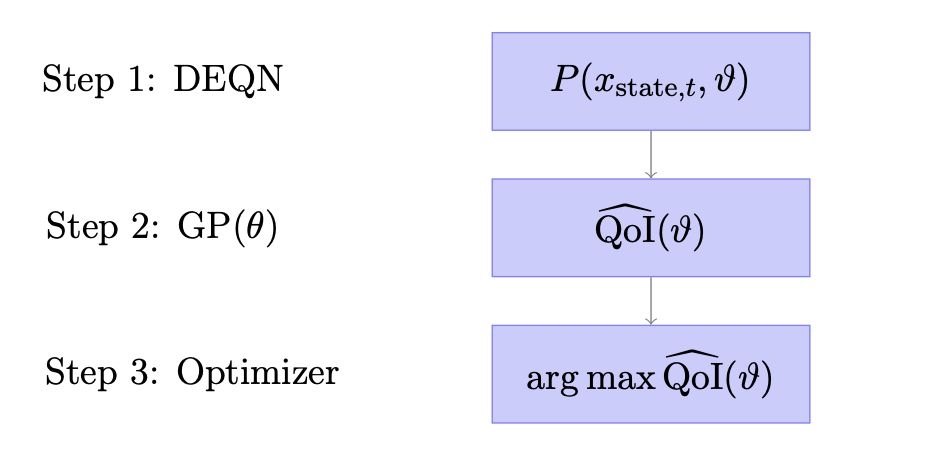
\includegraphics[width=0.72\textwidth]{tax/flow_chart_2.png}
 \end{figure}
 \vspace{-0.4em}
 \begin{center}
 \small The final box branches into the three operators: \emphc{estimate} ($\argmin$, Lecture 2) $\cdot$ \emphc{design} (constrained $\argmax$, Part III) $\cdot$ \emphc{quantify} (global sensitivity analysis, Part IV).
 \end{center}
\end{frame}

% --- What scales up ---
\begin{frame}{What Scales Up Relative to Lecture 2}
\footnotesize
\begin{center}
\begin{tabular}{p{0.21\textwidth}p{0.33\textwidth}p{0.36\textwidth}}
\toprule
 & \textbf{Lecture 2 (Brock--Mirman)} & \textbf{Today (climate applications)} \\
\midrule
Surrogate 1 inputs & state plus estimation pseudo-states & OLG IAM state $[t, TP_t, TP_{\mathrm{reached}}, \kappa_t, a_{t,j}, E_t]$ plus 16 policy pseudo-states (Part III); CDICE state plus uncertain $\bm{\theta}$ (Part IV) \\[3pt]
QoI shape & a few scalar moments & 40 cohort welfares (Part III) and an SCC surface $\mathrm{SCC}(\bm{\theta})$ (Part IV) \\[3pt]
Second surrogate & none needed: moments were cheap & GP regression + Bayesian active learning: each welfare evaluation costs 10{,}000 simulated paths \\
\bottomrule
\end{tabular}
\end{center}
\vspace{0.4em}
\textbf{Cost that does not scale up:} Surrogate 1 trains in about 4h from scratch on a laptop, minutes when warm-started; Surrogate 2 needs only 500 simulations (450 Latin hypercube + 50 actively learned).

\vspace{0.3em}
{\footnotesize \emph{Recaps if needed:} DEQNs --- Lecture 1; GP regression and Bayesian active learning --- Lecture 2 (Part 2).}
\end{frame}

% --- Operators formally ---
\begin{frame}{Post-Processing: Three Operators, Formally}
\footnotesize
\textbf{Estimate (Lecture 2, for continuity).}
\[
    \widehat\theta_{\text{SMM}} \;=\; \argmin_{\theta} \;
        \bigl[\widehat g_T - \widehat m_S(\theta)\bigr]^{\!\top}\, W \;
        \bigl[\widehat g_T - \widehat m_S(\theta)\bigr]
\]
\textbf{Design (Part III).} For a welfare QoI over policy parameters $\vartheta$:
\[
   \vartheta^* = \argmax_{\vartheta} \widehat{\mathrm{QoI}}(\vartheta)
   \quad \text{s.t. feasibility and, if imposed, Pareto constraints.}
\]
\textbf{Quantify (Part IV).} For a QoI $Y = \mathcal{M}(\bm{\theta})$ with uncertain $\bm{\theta} \sim p(\bm{\theta})$:
\begin{center}
\resizebox{0.94\textwidth}{!}{$\displaystyle
  \underbrace{\mathcal{M}^{1}_{i}(t) = \mathbb{E}_{\theta_{-i}}\!\left[ Y \mid \theta_{i}=t \right]}_{\text{univariate effect}}
  \qquad
  \underbrace{S_{i} = \frac{\mathrm{Var}_{\theta_{i}}\!\left[ \mathbb{E}\left[ Y \mid \theta_{i} \right] \right]}{\mathrm{Var}\left[ y \right]}, \quad
  S^{T}_{i} = \frac{\mathbb{E}_{\theta_{-i}}\!\left[\mathrm{Var}\left[ Y \mid \theta_{-i} \right]\right]}{\mathrm{Var}\left[ y \right]}}_{\text{first-order and total Sobol' indices}}
  \qquad
  \underbrace{Sh_{i}}_{\substack{\text{Shapley value: fair attribution} \\ \text{of } \mathrm{Var}(\mathrm{QoI}) \text{ across parameters}}}
$}
\end{center}
\vspace{0.1em}
Same surrogate under all three operators; only the question changes.
\end{frame}

% --- Today's instantiations ---
\begin{frame}{Today's Two Instantiations}
\begin{block}{Part III: Design}
$\vartheta$ = tax and transfer parameters $\cdot$ QoI = 40 cohort welfares $\cdot$ operator = constrained $\argmax$.
\end{block}
\vspace{0.8em}
\begin{block}{Part IV: Quantify}
$\bm{\theta}$ = structural parameters (preferences, damages, climate sensitivity) $\cdot$ QoI = the social cost of carbon $\cdot$ operator = global sensitivity analysis.
\end{block}
\end{frame}


% ============================================================================
% PART III: DESIGN --- CONSTRAINED OPTIMAL CARBON TAXES
% ============================================================================

% --- Section divider ---
\begin{frame}{}
\vfill
\begin{center}
{\Huge \textcolor{uzhblue}{\textbf{Part III}}}\\[12pt]
{\LARGE Design: Optimal Carbon Taxes and Transfers}\\[8pt]
{\small K\"ubler, Scheidegger \& Surbek (2026), \emph{Journal of Political Economy: Macroeconomics}}
\end{center}
\vfill
\end{frame}

% --- Motivation: designing optimal policy ---
\begin{frame}{Motivation: Designing Optimal Policy}
\begin{itemize}
    \setlength\itemsep{1.5em}
    \item \textbf{The Consensus:} Carbon pricing is widely regarded as the most efficient tool to mitigate emissions.
    \item \textbf{The Difficulty:} In a world with heterogeneous agents (e.g., OLG), simple taxes create winners and losers, threatening political feasibility.
    \item \textbf{The Objective:} We need a systematic way to compute \keyc{constrained optimal taxes} that:
    \begin{itemize}
        \item Account for stochastic risks (tipping points).
        \item Respect political constraints (Pareto improvements).
    \end{itemize}
\end{itemize}
\end{frame}

% --- The gap: welfare analysis in stochastic OLG IAMs ---
\begin{frame}[fragile]{The Gap: Welfare Analysis in Stochastic OLG IAMs}
\begin{figure}
    \centering
    
\includegraphics[width=0.45\linewidth]{tax/olg_agents.jpg}
    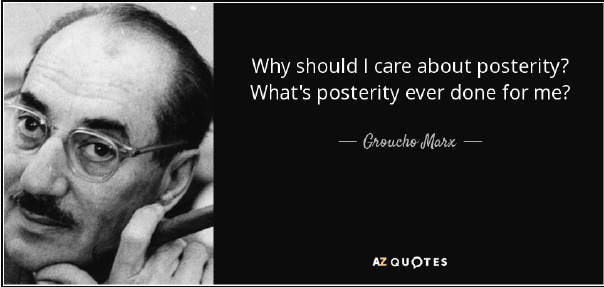
\includegraphics[width=0.45\linewidth]{tax/quote.png}
    \caption{Overlapping Generations.}
\end{figure}

\vspace{-0.2cm}

\begin{itemize}\small
    \setlength\itemsep{0.6em}
    \item \textbf{Current Limitations:} Most climate-macro research relies on \keyc{simplifying assumptions} (e.g., representative agents) or heuristic ``guessing'' to find Pareto improvements.
    \item \textbf{The Missing Tool:} A framework for \keyc{global solutions} in high-dimensional, stochastic environments that explicitly handles:
    \begin{itemize}
        \item \textbf{Heterogeneity:} Winners vs. Losers.
        \item \textbf{Uncertainty:} Tipping points and damage shocks.
    \end{itemize}
\end{itemize}
\end{frame}

% --- IAM primer ---
\begin{frame}{Integrated Assessment Models (IAMs)}
{\small Lecture 2's CDICE was one instantiation; here is the general recipe before we build a heterogeneous-agent one.}
\begin{itemize}\small
    \item Pioneered by Nordhaus (DICE, RICE): Quantitative, often numerical.
    \item Key components:
    \begin{itemize}
        \item (Simplified) climate system.
        \item (Stylized) economic model of emissions AND damages.
    \end{itemize}
    \item Economic model: needs to be dynamic, forward-looking, possibly allowing stochasticity (temperature variations, disasters, TFP), and potentially heterogeneous agents (``who is how impacted?'').
\end{itemize}
\vfill
\begin{figure}[h]
\centering
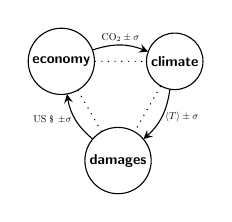
\begin{tikzpicture}[>=stealth, node distance=2cm, scale=0.36, transform shape]
    % Define style for the nodes
    \tikzstyle{main node} = [circle, draw, minimum size=1cm, font=\sffamily\Large\bfseries]

    % Nodes
    \node[main node] (economy) at (0,0) {economy};
    \node[main node] (climate) at (4,0) {climate};
    \node[main node] (damages) at (2,-3.5) {damages};

    % Arrows with labels
    \draw[->] (economy) to[bend left=20] node[above] {CO$_2 \pm \sigma$} (climate);
    \draw[->] (climate) to[bend left=20] node[right] {$\langle T \rangle \pm \sigma$} (damages);
    \draw[->] (damages) to[bend left=20] node[left] {US \$ $\pm \sigma$} (economy);

    % Triangle
    \draw[dotted] (economy) -- (climate) -- (damages) -- (economy);
\end{tikzpicture}
\caption{Stylized representation of an IAM.}
\label{fig:IAM_stylized}
\end{figure}
\end{frame}

% --- Overview of the stochastic IAM ---
\begin{frame}[fragile]{Overview of our Stochastic IAM}
{\small A \emphc{different IAM} from Lecture 2's CDICE: heterogeneous agents and a lean climate block, built for policy design.}
\begin{itemize}
    \item 12 Overlapping generations of selfish agents.
            \vspace{0.35cm}
    \item 5-yearly-calibrated model: agents live from age 20 to age 80.
            \vspace{0.35cm}
    \item Use a simple climate module~\citep{Dietz2020}.
            \vspace{0.35cm}
    \item Use a damage function with stochastic tipping~\citep{kotlikoffParetoimprovingCarbonriskTaxation2021a}.
            \vspace{0.35cm}
    \item Exogenously declining carbon intensity as in DICE-2016~\citep{nordhaus2017revisiting}.
\end{itemize}
\end{frame}

% --- Technology ---
\begin{frame}[fragile]{Technology}
\begin{footnotesize}
\keyc{Firms}, in each period, $t$, produce \keyc{final output, $Y_{t}$, and emissions $e_t$ with capital, $K_{t}$ and labor, $L_{t}$}, and choose how much of its emissions to \keyc{mitigate $\mu_t$} according to
\begin{equation} \label{eqFinalOutput}
(Y_t, e_t) = (\Omega_t(T_{t}) \Phi(\mu_t)
 K_t^{\alpha} L_t^{1-\alpha} + (1- \delta) K_t, \; \kappa_t (1-\mu_t)
 K_t^{\alpha} L_t^{1-\alpha})
\end{equation}
\begin{footnotesize}
    \begin{itemize}
\item $\Omega_t(T_{t})$: climate damages that reduce output.
\item $\Phi(\mu_t)$ is a mitigation cost function.
\item $\alpha$ is the capital share.
\item $\kappa_t$ is carbon intensity. We assume that $\kappa_t$ decreases stochastically over time as in \cite{kotlikoffParetoimprovingCarbonriskTaxation2021a}.
\item The abatement technology~\citep[{adapted from}][]{Nordhaus2017}: $\Phi(\mu_t) = (1-\theta_{1}\mu_t^{\theta_2})$.
\item $\theta_{1}$ and $\theta_2$ are parameters and $\mu_t \in [0, 1]$.
\end{itemize}
\end{footnotesize}
\vspace{0.3cm}
\keyc{Profit maximization} is given by:
\begin{equation}
    \begin{aligned}
        \max_{\mu_t, K_t, L_t} & \quad \Omega_t(T_{t}) (1-\theta_1\mu_t^{\theta_2}) K_t^{\alpha} L_t^{1-\alpha} + (1- \delta) K_t -w_tL_t-(1+r_t)K_t - \tau_t (1-\mu_t) \kappa_t K_t^{\alpha} L_t^{1-\alpha} \\
        \text{s.t.} & \quad 0 \leq \mu_t \leq 1.
    \end{aligned}
\end{equation}
\end{footnotesize}
\end{frame}

% --- Households ---
\begin{frame}[fragile]{Households}
\begin{footnotesize}
\begin{itemize}
    \item Agents enter the labor force at age 20 with 0 assets and die at age 80, after 12 periods.
    \item Agents born in period $t$ maximize lifetime utility:
    \begin{equation}
 {\mathbb E}_t \sum\limits_{j = 1}^{12} \beta^j \frac{C_{t+j-1, j}^{1-\sigma}}{1-\sigma} ,
\end{equation}
\begin{equation}
\text{subject to } C_{t,j}+a_{t+1, j+1}=(1+r_t)a_{t,j} +w_{t} l_{j} + \mathbb{T}_{t,j},
\end{equation}
where $C_{t,j}$, $a_{t,j}$, $l_{j}$ and $\mathbb{T}_{t,j}$ reference, respectively, \keyc{consumption, asset level, labor endowment, and transfer} of those born at time $t$ who are currently age $j$.
\item $l_{j}$ is similarly calibrated as in \cite{kotlikoff2021making}. \item Agents work for 8 periods, earning labor income, and then retire. Agents aged 9 to 12 work on a 40\% basis as a proxy for a state pension system.
\item $\beta$ is the discount factor and $\sigma$ is the coefficient of relative risk aversion.
\item Welfare criterion is
$$ U_t= {\mathbb E}_0  \sum\limits_{j = 1}^{12} \beta^j \frac{C_{t+j-1, j}^{1-\sigma}}{1-\sigma} $$
Use $ \tilde U_t $ for welfare under taxation.
\end{itemize}
\end{footnotesize}
\end{frame}

% --- Redistribution of tax income ---
\begin{frame}[fragile]{Redistribution of Tax Income}
\begin{itemize}
    \item Each period's tax income is redistributed to currently alive agents.
    \item In general, \keyc{transfer schemes may create winners and losers} \citep{kotlikoff2021making}.
    \item Today: \keyc{2 examples of transfer policies.}
    \begin{itemize}
        \item \keyc{``10\% scheme''}: The youngest generation receives the highest share of total tax income, with each older generation getting 10\% less than the next younger generation. Formally: $\mathbb{T}_{t,j} = 0.9^{(j-1)} \cdot 0.1394 \cdot \tau_t e_t, \quad j \in \{2,...,12 \}$.
        \vspace{0.5cm}
        \item \keyc{Optimal transfers}: Optimal transfer shares to each generation alive in a given period (fixed at $t=0$).
    \end{itemize}
\end{itemize}
\begin{itemize}
    \vspace{0.5cm}
    \item Normalization: Shares sum up to 1.
\end{itemize}
\end{frame}

% --- Cumulative emissions and temperature ---
\begin{frame}{Cumulative Carbon Emissions and Temperature}
\footnotesize
\textbf{Overview:} Climate science shows a near-linear link between cumulative CO$_2$ emissions and global temperature rise:
\begin{itemize}
    \item Global mean temperature increase ($T^{AT}_t$) is proportional to cumulative CO$_2$ emissions ($E_s$).
    \item The proportionality constant $\sigma_{CCR}$, known as the \keyc{Carbon-Climate Response (CCR) or TCRE}, \keyc{ranges from 1.0\,°C to 2.3\,°C per 1\,000 GtC (0.27\,°C to 0.63\,°C per 1\,000 GtCO$_2$)}.
\end{itemize}

\begin{columns}[c]
    \column{0.4\textwidth}
        \textbf{Equation:}
        \begin{equation}
            \label{eq:agg_emission}
            T^{AT}_t \approx \sigma_{CCR} \sum_{s=0}^{t} E_s
        \end{equation}
    \column{0.52\textwidth}
        \begin{figure}
            \centering
            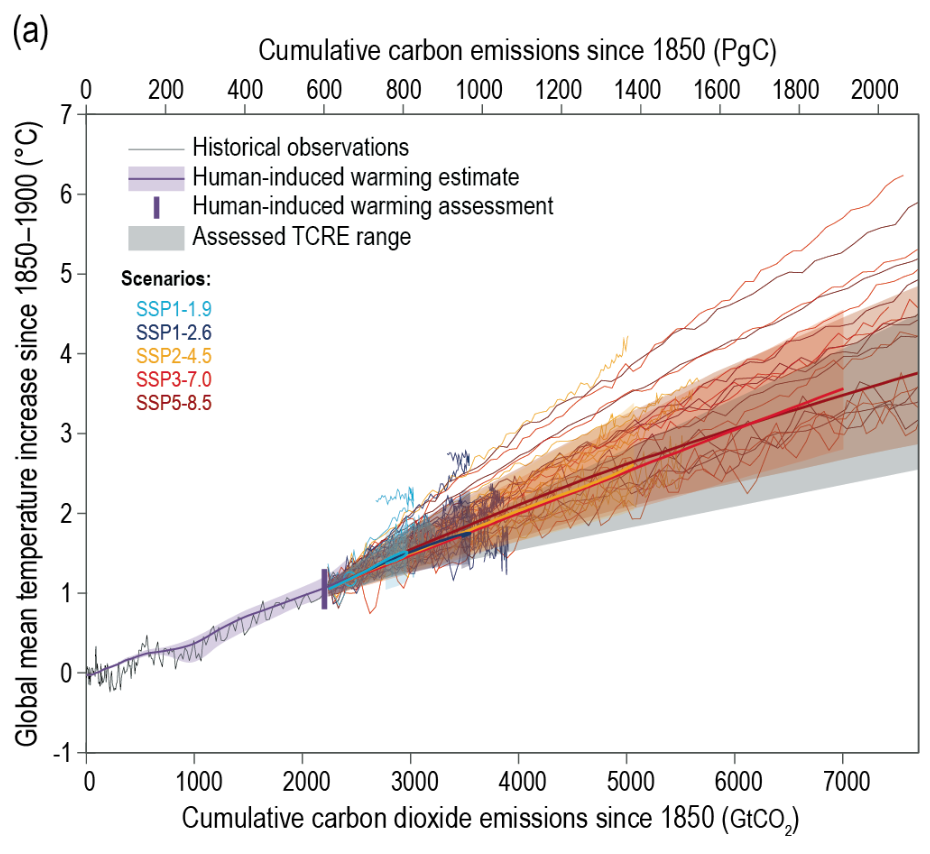
\includegraphics[width=0.28\linewidth]{tax/TCRS.png}
            \caption{Figure from IPCC 6.}
        \end{figure}
\end{columns}

\vspace{0.3em}
\textbf{Implications:}
\begin{itemize}
    \item Equation~\eqref{eq:agg_emission} is efficient and widely used in integrated assessment models (IAMs).
    \item It does not account for uncertainties in $\sigma_{CCR}$ nor for nonlinear effects such as potential tipping points (cf.\ Dietz and Venmans, 2019).
\end{itemize}
\end{frame}

% --- Damage function ---
\begin{frame}[fragile]{Damage Function}
\begin{small}
\begin{itemize}
    \item Damages reduce output.
    \item We include stochastic climate tipping as in \cite{weitzman2012ghg,kotlikoffParetoimprovingCarbonriskTaxation2021a}. Climate tipping is the occurrence of climate events that lead to irreversible damage to the environment (e.g., \citealp{lenton2008tipping}).
    \item The damage function takes the following form:
    \begin{equation}
        \label{eq:damage_func_tipping}
    \Omega_t \left( T_{ t} \right) =  \frac{1}{1 + \left(\frac{1}{\psi_1} T_{ t} \right)^{2} + \left( \frac{1}{2 \cdot TP_{t}} T_{ t} \right)^{6.754}}
    \end{equation}
    where $\psi_1$ is a damage parameter and $TP_t$ follows a random walk which is truncated at $TP_t \in [2.5, 3.5]$.
    \item Once the temperature hits a tipping point, $TP_t$ stays at the given level.
\end{itemize}
\end{small}
\end{frame}

% --- Uncertainty: shock processes ---
\begin{frame}[fragile]{Uncertainty}
\small
\begin{itemize}
    \item $\kappa_t$ follows an AR(1) process $\kappa_t = \rho_t \kappa_{t-1} + \epsilon_{\kappa,t}$ with $\kappa_0 = 0.3502$ and $\rho_t =  \rho_0 + (\rho_\infty - \rho_0) (1-\exp(- \delta^\rho  5t))$.
   \item $\epsilon_{\kappa,t}$ is discretized as:
    \begin{equation}
        \epsilon_{\kappa, t} =
\begin{cases}
0.03 & \text{with prob } 1/3, \\
0.0 & \text{with prob } 1/3, \\
- 0.03 & \text{with prob } 1/3.
\end{cases}
    \end{equation}
    \item $TP_t$ follows a random walk $TP_t = TP_{t-1} + \epsilon_{TP,t}$ with $TP_0 = 3.0$, $\epsilon_{TP,t}$ is discretized as:
    \begin{equation}
        \epsilon_{TP, t} =
\begin{cases}
0.1 & \text{with prob } 1/3, \\
0 & \text{with prob } 1/3, \\
- 0.1 & \text{with prob } 1/3.
\end{cases}
    \end{equation}
\end{itemize}
\end{frame}

% --- Equilibrium conditions ---
\begin{frame}[fragile]{Equilibrium Conditions}
{\footnotesize This system defines the DEQN loss for today's application --- the Lecture 1 recipe, applied to a new $\mathbf{G}$.}
\begin{footnotesize}
  \begin{columns}[t]
        \begin{column}{0.5\textwidth}
        \textbf{Firm:}
            \begin{align}
                0 & = \tau_t \kappa_t  - \Omega_t (T_{\mathrm{AT}, t}) \theta_1 \theta_2 \mu_t^{\theta_2 -1} \tag{$\mu_t$}\\
                r_t & = \left( \Omega_t (T_{\mathrm{AT}, t}) (1 - \theta_1 \mu_t^{\theta_2}) \right. \notag \\
                    & \quad \left. - \tau_t \kappa_t (1 - \mu_t) \right) \alpha K_t^{\alpha - 1} L_t^{1 - \alpha} - \delta \tag{$K_t$}\\
                w_t & = \left( \Omega_t (T_{\mathrm{AT}, t}) (1 - \theta_1 \mu_t^{\theta_2}) \right. \notag\\
                    & \quad \left. - \tau_t \kappa_t (1 - \mu_t) \right) (1 - \alpha) K_t^{\alpha} L_t^{-\alpha} \tag{$L_t$}
            \end{align}
            \textbf{Households:}

            For all households $j \in 1,...,A-1$:
            \begin{align}
                c_t^{-\sigma}  = \beta \mathbb{E}_t \left[ (1+ r_{t+1}) c_{t+1,j+1}^{-\sigma} \right] \tag{EE} \\
                C_{t,j} + a_{t+1, j+1}  =  (1 + r_t) a_{t,j} + w_{t} l_{t,j} + \mathbb{T}_{t,j}  \tag{BC}
            \end{align}
            and initial/final conditions $a_{t,1} = 0$, $a_{t+1,A} = 0$.
        \end{column}
        \begin{column}{0.5\textwidth}
            \textbf{Market Clearing:}
            \begin{align}
                K_t & = \sum_{j = 1}^{A} a_{t,j} \tag{$K_t$}\\
            L_t & = \sum_{j = 1}^{A} l_j \tag{$L_t$} \\
            \tau_{t} e_t & = \sum_{j=1}^{A} \mathbb{T}_{t,j}  \tag{$\mathbb{T}$}
            \end{align}
        \end{column}
  \end{columns}
\end{footnotesize}
\end{frame}

% --- Planner problem ---
\begin{frame}[fragile]{The Planner's Problem}
\small
\begin{itemize}
    \setlength\itemsep{0.8em}
    \item \textbf{Objective:} The planner chooses policy parameters $\vartheta$ (taxes \& transfers) to maximize the Social Welfare Function $\mathcal{W}$:
    \begin{align}
       \max_{\vartheta} \quad & \mathcal{W}(\vartheta) = \sum_{t = -10}^{30} \gamma_t \tilde{U}_t(\vartheta) \\
       \text{s.t.} \quad & \tilde{U}_t(\vartheta) \ge U_t \quad \forall t \quad \text{(if Pareto constrained)} \nonumber
    \end{align}
    \vspace{-0.5em}
    {\footnotesize (Where $\tilde{U}_t(\vartheta)$ is the ex-ante expected lifetime utility of generation $t$)}
    \item \textbf{Welfare Metric:} Gains are reported as the consumption equivalence factor ($\text{CE}_t$):
    \[
       \text{CE}_t = \left(\frac{\tilde{U}_t}{U_t}\right)^{\frac{1}{1-\sigma}}-1 \quad \text{\small{(where $U_t$ is business-as-usual (BAU) utility)}}
    \]
    \item \textbf{Scope \& Challenge:}
    \begin{itemize}
        \item Horizon: 40 generations (11 current, 29 future).
        \item Complexity: Solving for the optimal high-dimensional vector $\vartheta$ in a stochastic setting.
    \end{itemize}
\end{itemize}
\end{frame}

% --- Mapping OLG to DEQN ---
\begin{frame}[fragile]{Mapping the OLG Model to DEQN}
\noindent\textbf{Goal:} Approximate the policy functions of the OLG model using a neural network: the pseudo-state recipe of Lecture 2, scaled up.

\vspace{0.2cm}
\begin{columns}
\begin{column}{0.55\textwidth}
\textbf{Inputs (state vector):}
\begin{center}
\resizebox{0.96\linewidth}{!}{$
x = \big[t,\; TP_t,\; TP_{\mathrm{reached}},\; \kappa_t,\; a_{t,j},\; E_t,\;
\textcolor{uzhblue}{\vartheta}\big]
\in \mathbb{R}^{A + 5 + d_\vartheta}
$}
\end{center}
\textbf{Outputs (policy vector):}
\[
y = \big[a_{t+1,j+1},\; v_{t,j}\big]
\in \mathbb{R}^{2(A-1)}
\]
\textbf{Policy map:}
\[
\Pi: x \;\Rightarrow\; y
\]
\end{column}
\begin{column}{0.42\textwidth}
\textbf{Pseudo-states $\boldsymbol{\vartheta}$:}
\begin{itemize}
  \item $d_\vartheta = 16$: 4 tax parameters + 12 transfer shares.
  \item \keyc{DEQN learns policies for all tax rules and transfers at once}.
\end{itemize}
\vspace{0.3cm}
\textbf{Performance:}
\begin{itemize}
  \item Runtime from scratch: $\approx$4h on laptop.
  \item Warm start: a few minutes.
  \item Accuracy: MSE $\sim 10^{-6}$,\newline
  EE $\sim 10^{-3}$.
\end{itemize}
\end{column}
\end{columns}
\end{frame}

% --- Approximating welfare with surrogates ---
\begin{frame}{Approximating Welfare with Surrogates}
\footnotesize
    \textbf{The Computational Bottleneck:}
    \begin{itemize}\itemsep1pt
        \item DEQN solves the equilibrium, but evaluating expected welfare $\mathbb{E}[\mathcal{W}]$ requires expensive Monte Carlo simulations (10,000 paths per policy $\vartheta$).
        \item \textbf{Solution:} Train a \keyc{Gaussian Process (GP)} to map policy parameters $\vartheta$ directly to welfare outcomes.
    \end{itemize}
    \vspace{0.1em}
    \textbf{Two Optimization Targets (QoIs):}
    \begin{columns}[t]
        \begin{column}{0.48\textwidth}
            \begin{block}{1. Maximize Aggregate Welfare}
                \footnotesize
                \textbf{Goal:} Maximize scalar $\mathcal{W}$: \; $\max_\vartheta \mathbb{E}_0[\mathcal{W}(\vartheta)]$
                \begin{itemize}
                    \item \textbf{Surrogate:} Single scalar GP.
                    \item \textbf{Implication:} Ignores distribution (allows losers).
                \end{itemize}
            \end{block}
        \end{column}
        \begin{column}{0.48\textwidth}
            \begin{block}{2. Pareto Improvement}
                \footnotesize
                \textbf{Goal:} Maximize $\mathcal{W}$ subject to $\tilde{U}_t(\vartheta) \ge U_t \;\; \forall t$
                \begin{itemize}
                    \item \textbf{Surrogate:} Vector of 40 GPs (one per cohort).
                    \item \textbf{Implication:} No generation is worse off.
                \end{itemize}
            \end{block}
        \end{column}
    \end{columns}
\end{frame}

% --- Constructing the welfare surrogate ---
\begin{frame}{Constructing the Welfare Surrogate}
    \begin{columns}[t]
        \begin{column}{0.32\textwidth}
            \begin{block}{1. The Mapping}
                \footnotesize
                We map policy rules directly to \textbf{Expected Welfare}:
                \[
                    \vartheta \longmapsto \mathbb{E}_0[\mathcal{W}(\vartheta)]
                \]
                \begin{itemize}
                    \item \textbf{Input ($\vartheta$):} Tax and transfer parameters.
                    \item \textbf{Target:} Monte Carlo mean of lifetime utilities.
                \end{itemize}
            \end{block}
        \end{column}
        \begin{column}{0.32\textwidth}
            \begin{block}{2. Active Training}
                \footnotesize
                We populate the training set $\mathcal{D}$ efficiently:
                \begin{itemize}
                    \item \textbf{Initial Design:} 450 points sampled randomly (Latin Hypercube).
                    \item \textbf{Refinement:} 50 points added via \keyc{Bayesian Active Learning (BAL)}.
                    \item \textbf{Total:} Only 500 simulations needed.
                \end{itemize}
            \end{block}
        \end{column}
        \begin{column}{0.32\textwidth}
            \begin{block}{3. The Model}
                \footnotesize
                Fitting the Gaussian Process:
                \begin{itemize}
                    \item \textbf{Kernel:} Squared Exponential with Automatic Relevance Detection (ARD).
                    \item \textbf{Accuracy:} Leave-One-Out (LOO) error $\approx \mathbf{10^{-4}}$.
                    \item \textbf{Result:} A smooth, cheap-to-query surface.
                \end{itemize}
            \end{block}
        \end{column}
    \end{columns}

\vspace{0.2em}
{\footnotesize \emph{The GP + BAL machinery is exactly Lecture 2 (Part 2). Robustness:} training is anchored on a handful of trusted reference solutions to avoid \emph{lazy learning} --- the flat-in-the-parameter failure mode; 10--20 anchors suffice \citep{friedlDeep2023}.}
\end{frame}

% --- Maximizing welfare ---
\begin{frame}{Maximizing Welfare}
\small
\begin{itemize}
    \item We now have a cheap-to-evaluate surrogate model to map \keyc{tax functions onto welfare}. But we still need to find the optimal tax.
    \vspace{0.15cm}
    \item We aim to \keyc{find the $\argmax$ of our surrogate model}, which gives us the optimal tax function parameters:
    \[
       \vartheta^* = \argmax_{\vartheta} \widehat{\mathrm{QoI}}(\vartheta)
    \]
    s.t. various constraints.
    \vspace{0.15cm}
    \item We use \keyc{constrained optimization with linear constraints} for periods \{0,T\} that ensure that the parameters of the tax function stay within the feasible range during optimization.
    \end{itemize}
\vspace{0.15cm}
\begin{block}{Callback to Lecture 2}
Same object as the SMM criterion, opposite sign of intent: there we minimized distance to data, here we maximize welfare.
\end{block}
\end{frame}

% --- Calibration ---
\begin{frame}[fragile]{Calibration}
\vspace{-0.2em}
\begin{table}[]
    \centering
    \footnotesize
    \begin{tabular}{ccc}
    \hline \hline
  \textbf{Symbol} & \textbf{Parameter} & \textbf{Value} \\
    \hline
    $\beta$  & Discount factor& 0.9 \\
    $\sigma$  & Relative risk aversion & 3 \\
    $\alpha$  & Capital share & 0.3 \\
    $\delta$  &Depreciation & 0.2 \\
    $\sigma_{ccr}$  & Climate sensitivity & 1.7 \\
    $\psi_1$  & parameter damage function & 13.16 \\
    $\theta_1$  & Intercept of control cost function & 0.7 \\
    $\theta_2$  & Exponent of control cost function & 2.6 \\
    $\kappa_{0}$  & Initial carbon intensity & 0.35032 \\
    $\rho_0$  & Initial AR(1) param for carbon intensity & 1.08 \\
    $\rho_{\infty}$  & Final AR(1) param for carbon intensity & 0.91 \\
    $\delta^{\rho}$  & AR(1) param depreciation for carbon intensity  & 0.04 \\
    $E_0$ & initial stock of carbon thGtC& 0.851 \\
    $L$ & Labor (to match initial emissions) & 600 \\
    \hline
\end{tabular}
    \caption{Parameterization of the OLG Model.}
    \label{tab:parameters}
\end{table}
\end{frame}

% --- BAU vs RCP ---
\begin{frame}{BAU Scenario versus RCP Scenarios}
    \centering
    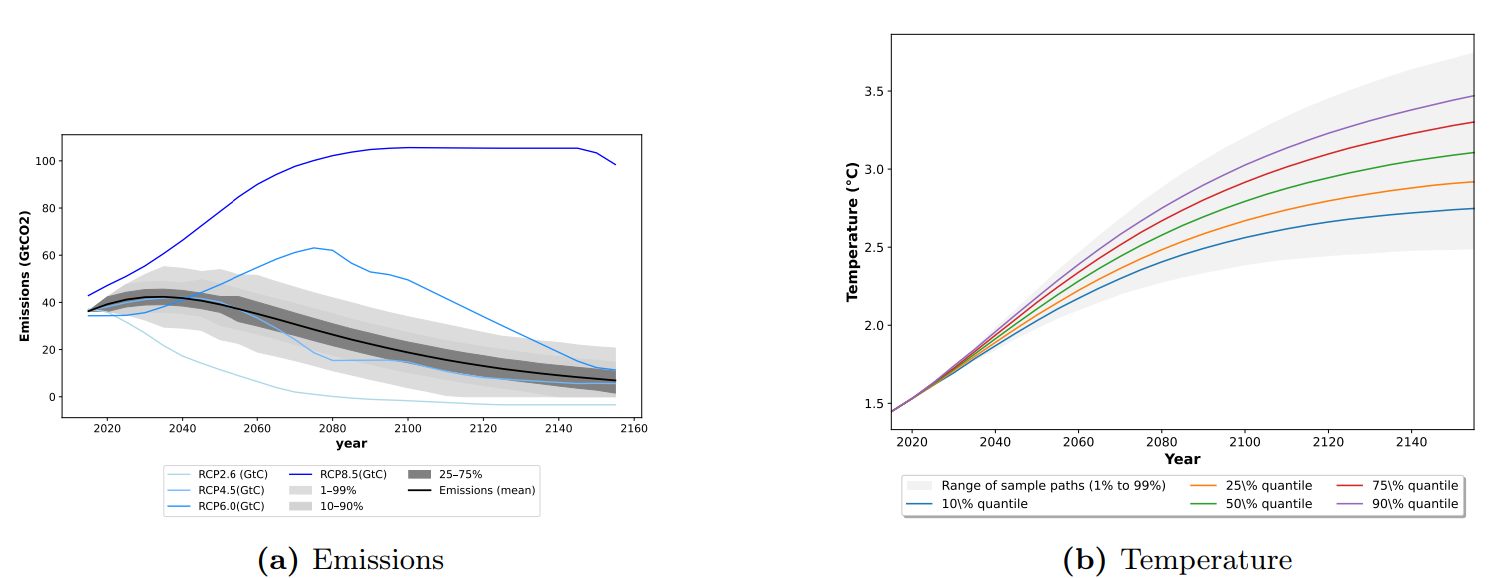
\includegraphics[width=0.7\textwidth, height=0.4\textheight, keepaspectratio]{tax/BAU_SOLG.png}

    \vspace{0.3em}
    \begin{columns}[t]
        \begin{column}{0.48\textwidth}
            \footnotesize
            \textbf{Left: Global CO$_2$ Emissions}
            \begin{itemize}
                \item Comparison of our model's BAU against IPCC Representative Concentration Pathways (RCP).
                \item Our endogenous emissions path tracks closely with \textbf{RCP 4.5}.
                \item Base year (0) corresponds to 2017.
            \end{itemize}
        \end{column}
        \begin{column}{0.48\textwidth}
            \footnotesize
            \textbf{Right: Global Warming Projections}
            \begin{itemize}
                \item Projected mean warming reaches $\approx \mathbf{3^\circ C}$ over 150 years.
                \item Substantial uncertainty exists: range of \textbf{2.5°C to 3.6°C}.
                \item Highlights significant tail risk in the absence of policy.
            \end{itemize}
        \end{column}
    \end{columns}
\end{frame}

% --- Three policy scenarios ---
\begin{frame}{Three Policy Scenarios}
\small
    \begin{itemize}
        \setlength\itemsep{1em}
        \item \textbf{Scenario 1: Unconstrained Welfare Maximization} \\
        \small{Linear tax on cumulative emissions + exogenous transfers.}
        \begin{equation*}
            \tau_t(E_t) = \vartheta_0 + \vartheta_E \cdot E_t
        \end{equation*}
        \item \textbf{Scenario 2: Pareto-Improving Policy} \\
        \small{Linear tax on cumulative emissions + \textbf{optimal} transfers.}
        \begin{equation*}
             \tau_t(E_t) = \vartheta_0 + \vartheta_E \cdot E_t
        \end{equation*}
        \item \textbf{Scenario 3: Increasing Policy Complexity} \\
        \small{Linear tax on cumulative emissions, carbon intensity ($\kappa$), and tipping risk ($TP$) + optimal transfers.}
        \begin{equation*}
            \tau_t(\cdot) = \vartheta_0 + \vartheta_E E_t + \vartheta_\kappa \kappa_t + \vartheta_{TP} (1-\mathbb{D}_{TP})
        \end{equation*}
    \end{itemize}
\end{frame}

% --- Scenario 1 ---
\begin{frame}{Scenario 1: Unconstrained Welfare Maximization}
\small
Each period's tax income is redistributed to currently alive agents; in general, \keyc{transfer schemes may create winners and losers} \citep{kotlikoff2021making}. Here: the ``10\% scheme''. The youngest generation receives the largest share of total tax revenue, and the share for each older generation decreases by 10\% relative to the next younger one. The shares are normalized to sum to one. Formally, our transfer scheme, $\mathbb{T}$, is defined as:
\begin{equation}
    \mathbb{T}_{t,j} = 0.9^{(j-1)} \cdot 0.1394 \cdot \tau_t e_t, \quad j \in \{2,...,12 \}.
\end{equation}
The resulting constrained optimization problem reads as:
\begin{equation}
\label{eq:optim_cum_emm_maxwelf}
\begin{aligned}
  \vartheta^{\ast}
  \;=\;
  & \arg\max_{\vartheta\in[a,b]}\,
  \widehat{\mathrm{QoI}}(\vartheta) \\
& \quad \text{s.t.} \\
& 0 \leq \vartheta_0 + \vartheta_E  E_0 \leq \bar{\tau}, \\
& 0 \leq \vartheta_0 + \vartheta_E  E_{29} \leq \bar{\tau}.
\end{aligned}
\end{equation}
\end{frame}

% --- Welfare surrogate (scenario 1) ---
\begin{frame}{The Welfare Surrogate (Scenario 1)}
\begin{columns}[c]
    \begin{column}{0.55\textwidth}
        \centering
        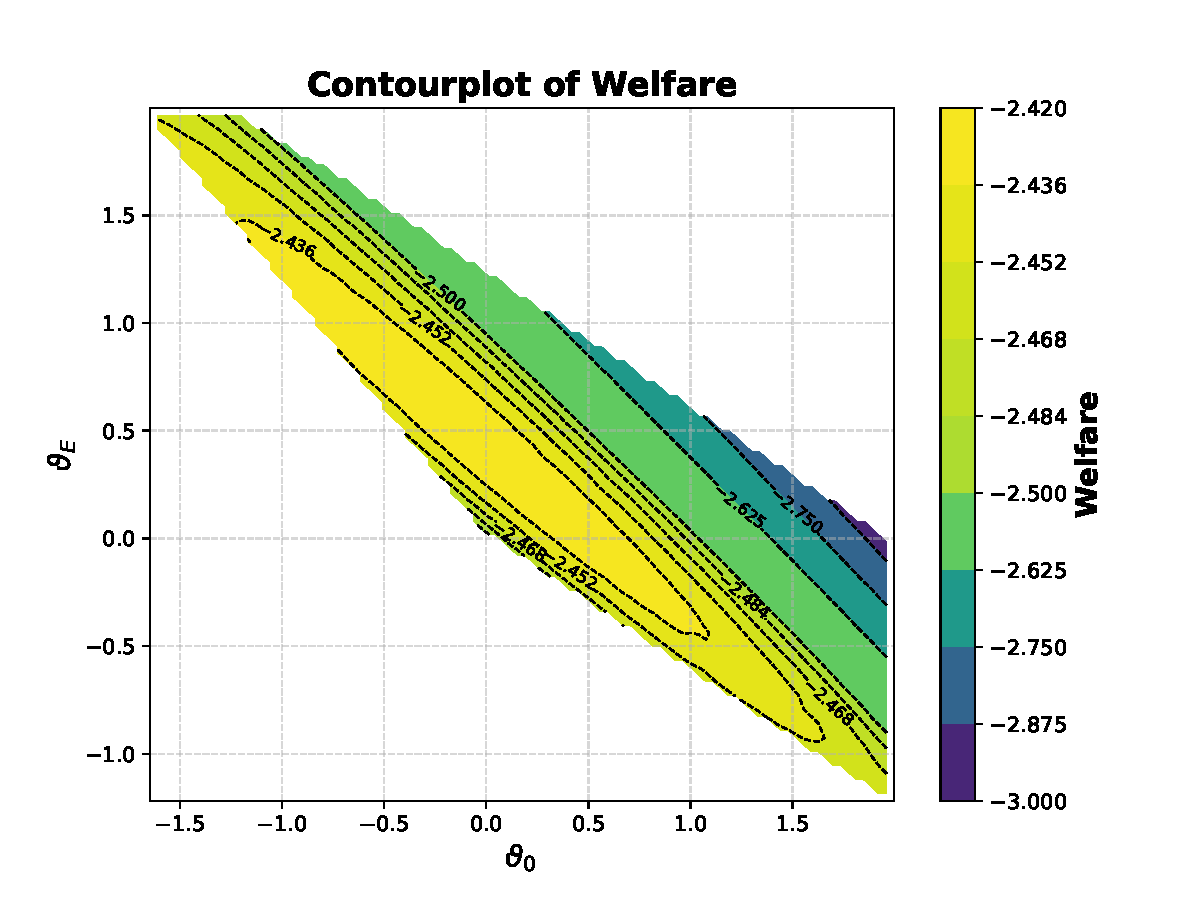
\includegraphics[width=0.92\linewidth]{tax/paper/contour_welfare_E.pdf}
    \end{column}
    \begin{column}{0.42\textwidth}
        \small
        \begin{itemize}
            \setlength\itemsep{1em}
            \item \textbf{The Surface:} A Gaussian Process approximation of the Social Welfare Function.
            \item \textbf{The Axes:} Tax Intercept ($\vartheta_0$) vs. Slope ($\vartheta_E$).
            \item \textbf{The Goal:} Find the ``peak'' (yellow zone) without running millions of simulations.
            \item \textbf{Precision:} Leave-One-Out error $\approx \mathbf{10^{-5}}$.
        \end{itemize}
    \end{column}
\end{columns}
\end{frame}

% --- Temperature (scenario 1) ---
\begin{frame}{Temperature (Scenario 1: Unconstrained)}
\begin{columns}[c]
    \begin{column}{0.5\textwidth}
        \centering
        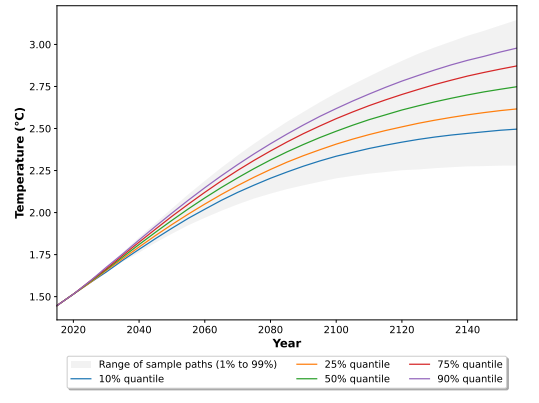
\includegraphics[width=0.92\linewidth]{tax/Temp_case1.png}
    \end{column}
    \begin{column}{0.47\textwidth}
        \small
        \textbf{Outcomes:}
        \begin{itemize}
            \setlength\itemsep{0.8em}
            \item \textbf{Aggressive Mitigation:} Stabilizes mean warming at \textbf{$\approx$2.7\,°C}.
            \item \textbf{Tail-Risk Insurance:} The 99th percentile is capped at $\approx$3.1\,°C.
            \item \textbf{The Mechanism:} Requires immediate, heavy taxation ($\approx$70\% average after 150 years).
            \item \textbf{The Cost:} Imposes up to \textbf{$-$5\% welfare losses} on current older cohorts.
        \end{itemize}
    \end{column}
\end{columns}
\end{frame}

% --- Emissions (welfare maximizing) ---
\begin{frame}{Emissions (Welfare Maximizing)}
\begin{columns}[c]
    \begin{column}{0.55\textwidth}
        \centering
        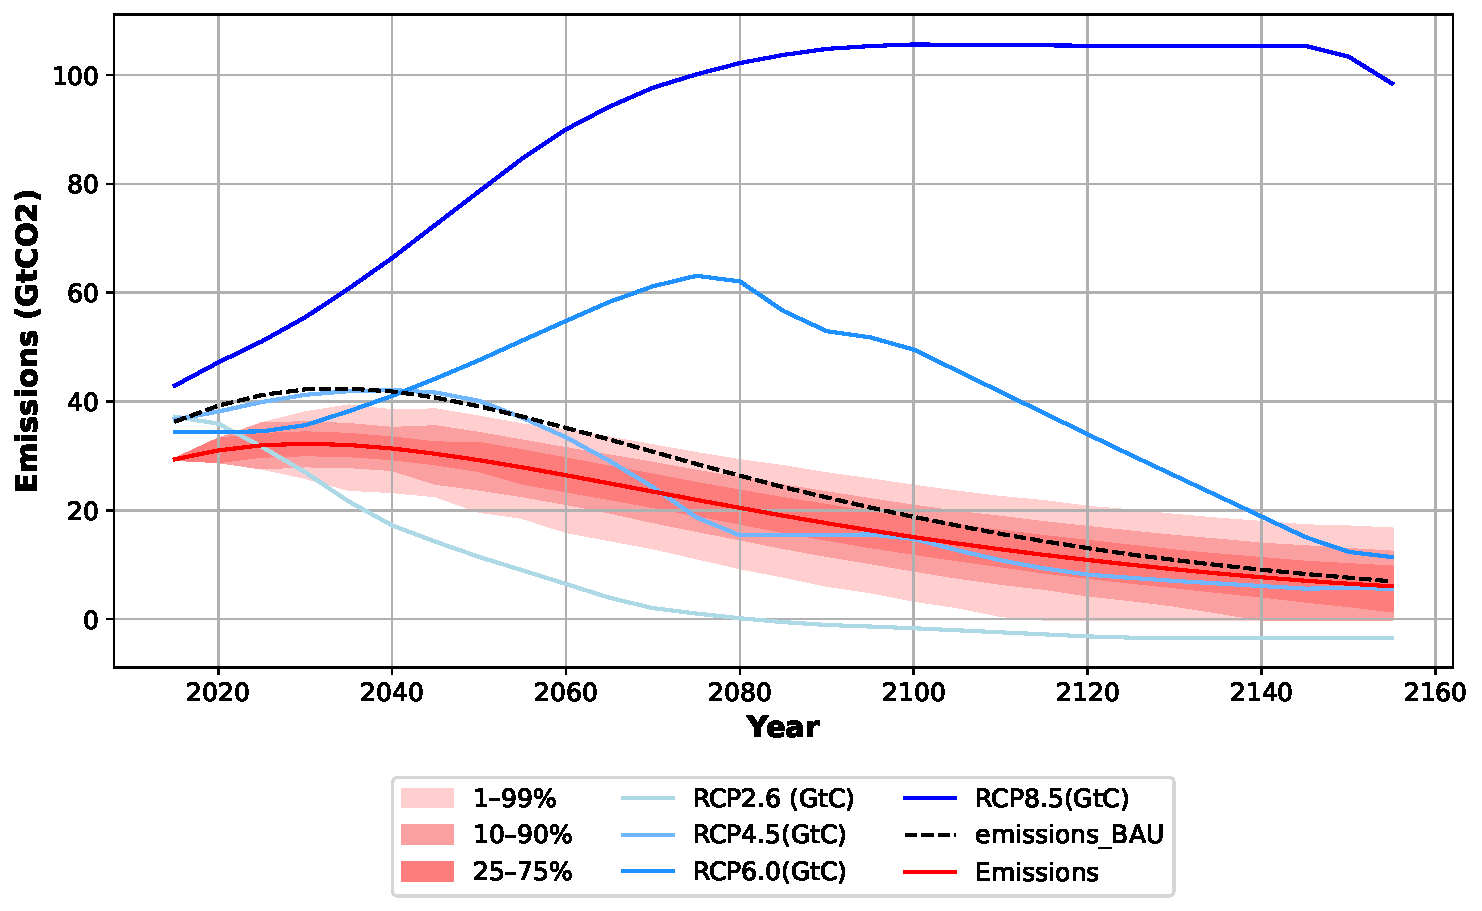
\includegraphics[width=0.92\linewidth]{tax/paper/lin_S_10trans_unif_emissions.pdf}
    \end{column}
    \begin{column}{0.42\textwidth}
        \small
        \begin{itemize}
            \setlength\itemsep{1em}
            \item \textbf{Immediate Shock:} Emissions drop $\approx \mathbf{25\%}$ below BAU within the first 50 years.
            \item \textbf{Eliminating the Extremes:} The policy successfully truncates the high-emission tail (the red shaded area).
            \item \textbf{Convergence:} Post-2100, the gap narrows as exogenous carbon intensity declines naturally.
        \end{itemize}
    \end{column}
\end{columns}
\end{frame}

% --- Optimal welfare distribution ---
\begin{frame}{Optimal Welfare Distribution}
\begin{columns}[c]
    \begin{column}{0.55\textwidth}
        \centering
        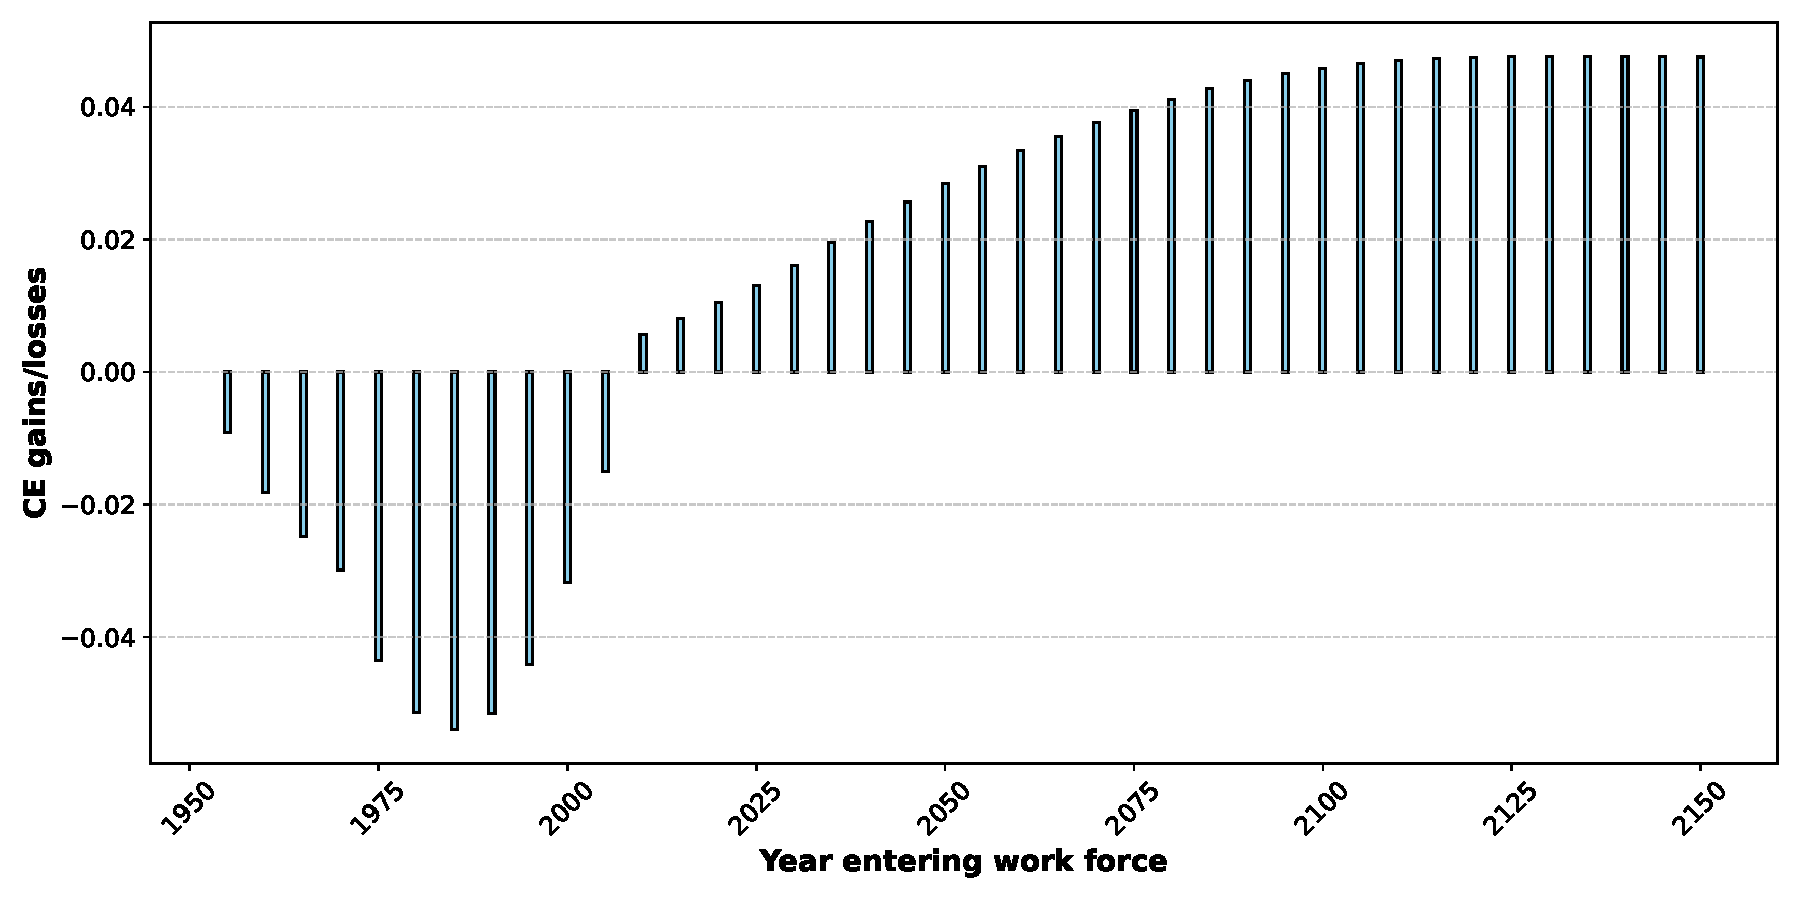
\includegraphics[width=0.92\linewidth]{tax/paper/lin_S_10trans_unif_welfares.pdf}
    \end{column}
    \begin{column}{0.42\textwidth}
        \small
        \textbf{The Price:}
        \begin{itemize}
            \setlength\itemsep{0.8em}
            \item \textbf{Aggregate Welfare Gain:} The total pie grows by \textbf{1.6\%} (consumption equivalent).
            \item \textbf{Future Gain:} Generations born after 2100 enjoy gains of $\approx \mathbf{4.8\%}$.
            \item \textbf{Current Pain:} \emphc{This comes at a steep cost.} Transition generations suffer losses up to \textbf{5\%}.
            \item \textbf{Conclusion:} Without transfers, this optimal policy is politically dead on arrival.
        \end{itemize}
    \end{column}
\end{columns}
\end{frame}

% --- The challenge (pivot to Pareto) ---
\begin{frame}{The Challenge}
\begin{itemize}
    \setlength\itemsep{1.2em}
    \item The welfare-maximizing tax (simple example) reduces warming to $2.7^\circ$C.
    \item \textbf{But:} It imposes welfare losses of up to \textbf{5\%} on current older generations.
    \item \textbf{Result:} The policy is economically efficient but politically infeasible.
    \item \textbf{Goal:} Can we design a tax \textit{and} transfer scheme where $\tilde{U}_t \ge U_t$ for all $t$?
\end{itemize}
\end{frame}

% --- Scenario 2 ---
\begin{frame}{Scenario 2: Pareto-Improving Policy}
\footnotesize
For 40 values of $t$:
\begin{equation}
    \mu_{*,t}(\vartheta) \;=\; \widehat{\mathrm{QoI}}_t(\vartheta)
  \;=\;
  \mathbb{E}\!\bigl[\tilde{U}_t(\vartheta)\bigr] \quad \forall \; t \in \{-10,...,29\}
\end{equation}
Solve:
\begin{equation}
\label{eq:opt_pareto_y2}
\begin{aligned}
  &\vartheta^{\ast}
  \;=\;
  \arg\max_{\vartheta\in[a,b]}
  \sum_{t=-10}^{29}\gamma_t\, \widehat{\mathrm{QoI}}_t(\vartheta)
  \;=\;
  \arg\max_{\vartheta\in[a,b]}
  \sum_{t=-10}^{29}\gamma_t\,\mathbb{E}_0\!\bigl[\tilde{U}_t(\vartheta)\bigr] \\
& \quad \text{s.t.} \quad
 \mathbb{E}_0\!\bigl[\tilde{U}_t(\vartheta)\bigr]
  \;\ge\;
  \mathbb{E}_0\!\bigl[U_t\bigr]
  \;\;\forall\,t, \\
& \phantom{\quad \text{s.t.} \quad} 0 \leq \vartheta_0 + \vartheta_E  E_0 \leq \Bar{\tau}, \qquad
 0 \leq \vartheta_0 + \vartheta_E  E_{29} \leq \Bar{\tau},  \qquad
 \sum_{i=1}^{12} \vartheta_i = 1
\end{aligned}
\end{equation}
\end{frame}

% --- Optimal parameters and transfers ---
\begin{frame}{Optimal Parameters and Transfers}
We find optimal tax parameters: $\vartheta_0 = -0.186$ and $\vartheta_E = 0.225$.\newline

The optimal transfer shares allocate resources to specific cohorts to satisfy the Pareto constraints:
\begin{table}[htbp]
\begin{footnotesize}
        \centering
    \begin{tabular}{|c|c|c|c|c|c|c|c|c|c|c|c|c|}
        \hline
        \textbf{t1} & \textbf{t2} & \textbf{t3} & \textbf{t4} & \textbf{t5} & \textbf{t6} & \textbf{t7} & \textbf{t8} & \textbf{t9} & \textbf{t10} & \textbf{t11} & \textbf{t12} \\
        \hline
        0.128 & 0.051 & 0.058 & 0.09 & 0.15 & 0.09 & 0.066 & 0.143 & 0.076 & 0.048 & 0.039 & 0.06 \\
        \hline
    \end{tabular}
    \caption{\textbf{Pareto optimal transfer scheme.} Optimal shares for each concurrent cohort $i$ under the linear cumulative emissions tax.}
    \label{tab:optimal_transfer_lin_S}
    \end{footnotesize}
\end{table}
\end{frame}

% --- Optimal welfare (Pareto) ---
\begin{frame}{Optimal Welfare (Pareto Improving)}
\begin{columns}[c]
    \begin{column}{0.55\textwidth}
        \centering
        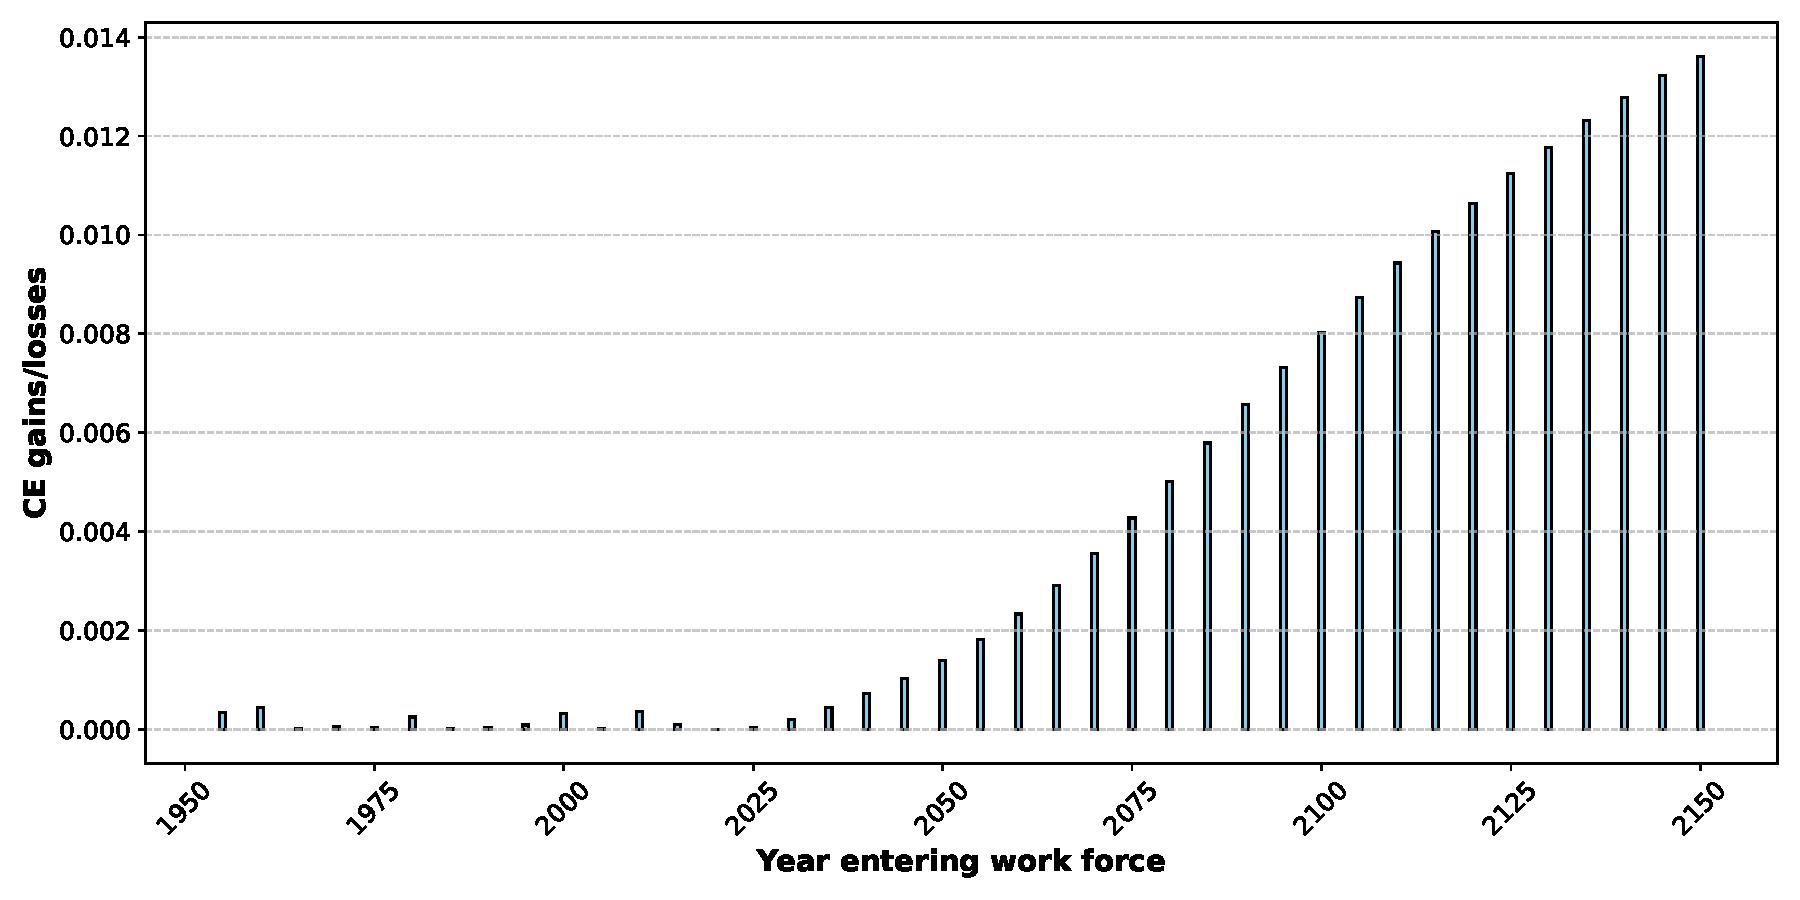
\includegraphics[width=0.92\linewidth]{tax/paper/welfare_gains_lin_S_trans.pdf}
    \end{column}
    \begin{column}{0.42\textwidth}
        \small
        \begin{itemize}
            \setlength\itemsep{0.8em}
            \item \textbf{The Pareto Constraint:} Transfers are explicitly optimized to keep initial generations (and those born in the next decade) at \textbf{BAU levels} (0\% loss).
            \item \textbf{Future Gains:} Welfare improves monotonically, reaching \textbf{$\approx$1.4\%} for distant generations.
            \item \textbf{The Cost of Consensus:} Compared to the unconstrained case (max 4.8\%), future gains are smaller, but \textbf{no generation loses}.
            \item \textbf{Aggregate:} Total welfare gain of \textbf{0.42\%}.
        \end{itemize}
    \end{column}
\end{columns}
\end{frame}

% --- Temperature (scenario 2) ---
\begin{frame}{Temperature (Scenario 2: Pareto-Improving)}
\begin{columns}[c]
    \begin{column}{0.5\textwidth}
        \centering
        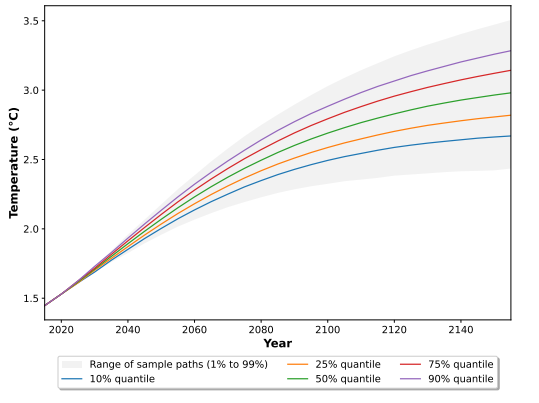
\includegraphics[width=0.86\linewidth]{tax/Temp_case2.png}
    \end{column}
    \begin{column}{0.47\textwidth}
        \small
        \begin{itemize}
            \setlength\itemsep{0.4em}
            \item \textbf{The Trade-off:} Mean warming settles just below \textbf{3\,°C} (higher than Scenario 1).
            \item \textbf{Crucial Insurance:} The 99th percentile \textbf{never exceeds 3.5\,°C}.
            \item \textbf{Tail Truncation:} The policy deliberately eliminates the catastrophic tail ($>$3.6\,°C under BAU).
            \item \textbf{The Win:} Achieved with optimal transfers $\to$ \textbf{no generation loses}.
            \item \keyc{\textbf{Conclusion:} The Pareto-optimal policy functions primarily as disaster insurance rather than aggressive mitigation.}
        \end{itemize}
    \end{column}
\end{columns}
\end{frame}

% --- Emissions (Pareto) ---
\begin{frame}{Emissions: Mitigating Risk (Scenario 2)}
\begin{columns}
    \begin{column}{0.55\textwidth}
        \begin{figure}[th!]
            \centering
            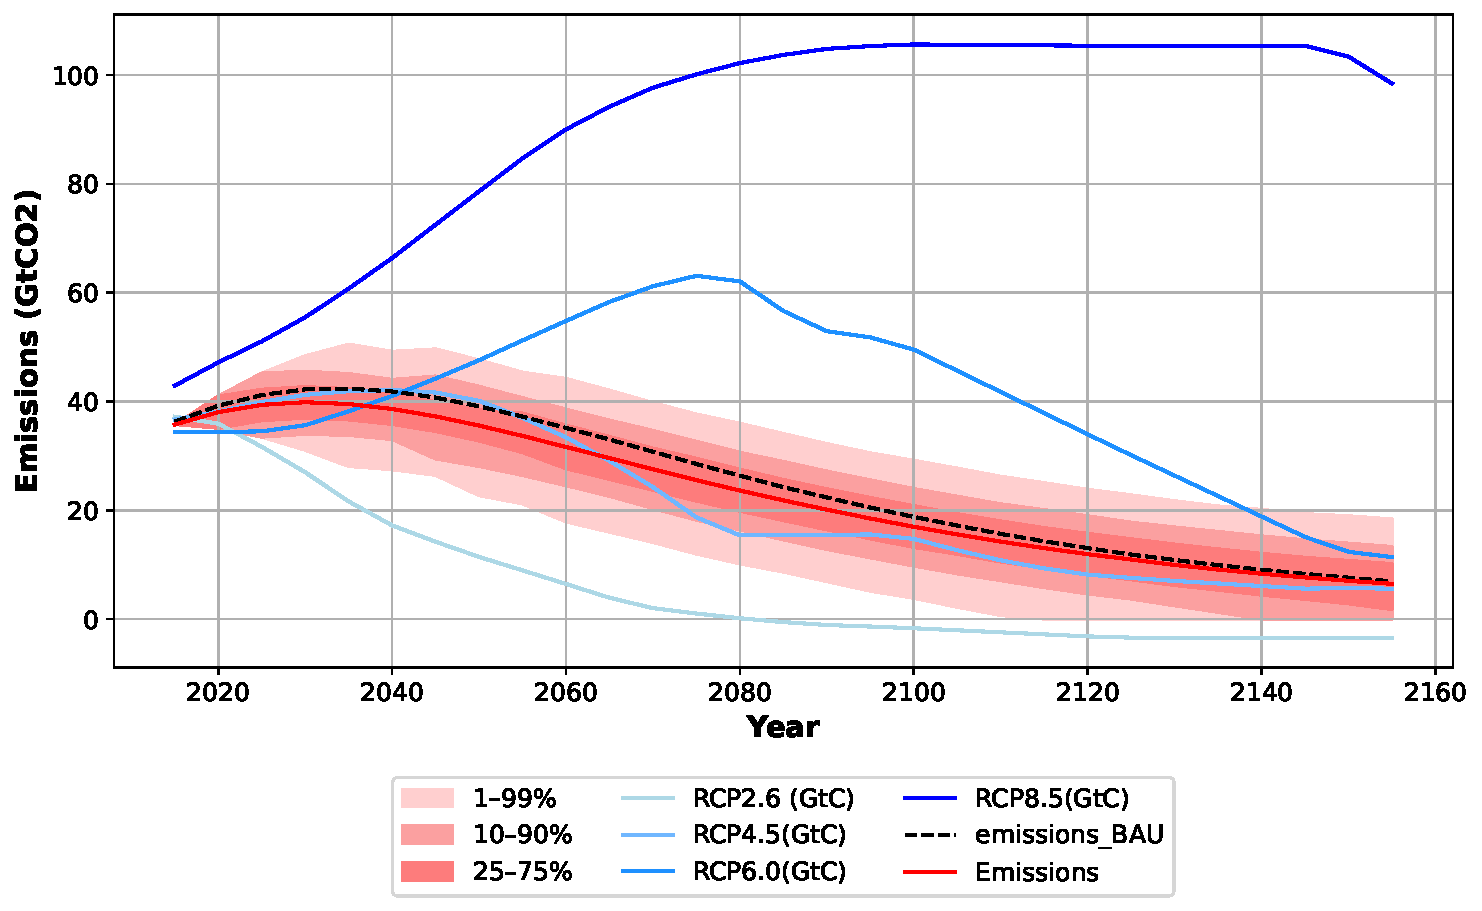
\includegraphics[width=0.92\linewidth]{tax/paper/lin_S_trans_emissions_dist.pdf}
        \end{figure}
    \end{column}
    \begin{column}{0.42\textwidth}
        \footnotesize
        \begin{itemize}
             \setlength\itemsep{0.9em}
            \item \textbf{Modest Average Reduction:} The mean emissions path is not drastically lower than BAU (required to preserve current consumption).
            \item \textbf{Tail Truncation:} The policy's primary physical impact is eliminating the high-emissions upside.
            \item \textbf{Result:} The $99^{th}$ percentile of emissions drops below $40~GtCO_2$ by 2070 (20 years earlier than BAU).
        \end{itemize}
    \end{column}
\end{columns}
\end{frame}

% --- Scenario 3 ---
\begin{frame}{Scenario 3: Increasing Policy Complexity}
\small
    \textbf{Question:} Can we improve welfare by targeting specific climate drivers?
    \vspace{0.5em}

    We expand the tax rule to include \textbf{Carbon Intensity} ($\kappa_t$) and \textbf{Tipping Risk} ($TP_t$):
    \begin{equation}
        \label{eq:tax_fun_lin_S_kappa_tipping}
        \tau_t = \vartheta_0 + \vartheta_E \frac{E_t}{E_0} + \underbrace{\vartheta_\kappa \frac{\kappa_t}{\kappa_0}}_{\text{Intensity}} + \underbrace{\vartheta_{TP} (1 - \mathbb{D}_{TP})}_{\text{Tipping Risk}}
    \end{equation}
    \begin{itemize}
        \item $\mathbb{D}_{TP} \in [0,1]$: Normalized distance to the tipping threshold.
        \item \textbf{Dimensionality:} This adds new pseudo-states, increasing the parameter space to $d_\vartheta = 16$ (4 tax parameters + 12 transfer shares).
        \item We use the same ML-based optimization to find the constrained Pareto-optimal policy.
    \end{itemize}
\end{frame}

% --- Diminishing returns ---
\begin{frame}{Results: Diminishing Returns to Complexity}
\small
    We find the optimal parameters:
    \[
        \{\vartheta_0, \vartheta_E, \vartheta_\kappa, \vartheta_{TP} \} = \{-0.237,\;  0.203, \;  0.037, \;  0.012 \}
    \]
    \textbf{Key Finding:} Complexity adds very little welfare value.
    \begin{table}[h]
        \centering
        \begin{tabular}{lcc}
            \toprule
            \textbf{Policy Specification} & \textbf{Instruments} & \textbf{Welfare Gain*} \\
            \midrule
            Linear in Cumulative Emissions ($E_t$) & 2 & \textbf{0.42\%} \\
            Linear in $E_t, \kappa_t, TP_t$ & 4 & \textbf{0.45\%} \\
            \bottomrule
        \end{tabular}
        \caption{\footnotesize Aggregate welfare gains in consumption-equivalent terms.}
    \end{table}
    \begin{alertblock}{Conclusion:}
        A simple, well-designed tax on cumulative emissions captures \textbf{93\%} of the potential welfare gains. Adding complex state-dependencies provides only marginal benefits.
    \end{alertblock}
\end{frame}

% --- Cost of political feasibility ---
\begin{frame}{The Cost of Political Feasibility}
\small
    Comparing the physical outcomes of the two approaches reveals a crucial trade-off: \newline
    \begin{columns}[t]
        \begin{column}{0.5\textwidth}
            \textbf{1. Welfare Maximizing} \\ (Unconstrained)
            \begin{itemize}
                \item \keyc{Aggressive early mitigation.}
                \item Warming stabilizes at $\mathbf{\approx 2.7^\circ C}$.
                \item \emphc{Current generations lose (up to 5\%).}
            \end{itemize}
        \end{column}
        \begin{column}{0.5\textwidth}
            \textbf{2. Pareto Improving} \\ (Constrained)
            \begin{itemize}
                \item \keyc{Slower initial mitigation path.}
                \item Warming stabilizes at $\mathbf{\approx 3.0^\circ C}$.
                \item \textcolor{darkgreen}{No generation loses.}
                \item \textbf{\textcolor{softorange}{Crucial: Truncates worst-case damages (insurance).}}
            \end{itemize}
        \end{column}
    \end{columns}
    \vspace{0.8em}
    \begin{alertblock}{Trade-off \& Insurance}
        Ensuring political support requires delaying some mitigation, leading to higher \textit{average} temperatures ($\approx +0.3^\circ C$). However, it successfully \textbf{eliminates extreme damage scenarios} ($>15\%$ of GDP), effectively insuring future generations against climate disasters.
    \end{alertblock}
\end{frame}


% ============================================================================
% PART IV: QUANTIFY --- DEEP UQ OF THE SOCIAL COST OF CARBON
% ============================================================================

% --- Section divider ---
\begin{frame}{}
\vfill
\begin{center}
{\Huge \textcolor{uzhblue}{\textbf{Part IV}}}\\[12pt]
{\LARGE Quantify: How Uncertain Is the Social Cost of Carbon?}\\[8pt]
{\small The \emph{quantify} operator on the same two-surrogate pipeline\\
Friedl, K\"ubler, Scheidegger \& Usui (2023)}
\end{center}
\vfill
\end{frame}

% --- Stochastic IAM with Bayesian learning ---
\begin{frame}
\frametitle{A Stochastic IAM with Learning about the ECS}
\vspace{-0.2em}
{\scriptsize Back to the global IAM of Lecture 2 (Part 1): CDICE, now with recursive (Epstein--Zin) utility, a stochastic equilibrium climate sensitivity (ECS), and Bayesian learning.\par}
\vspace{-0.2em}
\begin{center}
\resizebox{0.42\linewidth}{!}{
  \begin{minipage}{\linewidth}
\begin{align*}
  & V\left(\bm{X}_t\right)^{1-1/\psi}
  = \max_{C_{t},K_{t+1},\mu_{t}}\left\{\left( \frac{C_{t}}{L_{t}} \right)^{1-1/\psi}L_{t}
    +
    e^{-\rho} \mathbb{E}_{t}\left[V\left(\bm{X}_{t+1}\right)^{1-\gamma}\right]^{\frac{1-1/\psi}{1-\gamma}}\right\}
  \\
  \text{s.t.} \quad
  &
    \left(1-\Theta\left(\mu_{t}\right)\right)\Omega_t\left(T_{\mathrm{AT},t}\right)K_{t}^{\alpha}\left( A_{t}L_{t} \right)^{1-\alpha}
    - C_{t} - I_{t} = 0 \\
  &  \left( 1-\delta \right)K_{t} + I_{t} - K_{t+1} = 0\\
  &  1 - \mu_{t} \geq 0  \\
  &
  \left(1-\phi_{12}\right)M_{\mathrm{AT},t}+\phi_{21}M_{\mathrm{UO},t}+\left(1-\mu_{t}\right)\sigma_{t}K_{t}^{\alpha}\left( A_{t}L_{t} \right)^{1-\alpha} + E_{\mathrm{Land},t} - M_{\mathrm{AT},t+1} = 0 \\
      &
    \phi_{12}M_{\mathrm{AT},t}+\left(1-\phi_{21}-\phi_{23}\right)M_{\mathrm{UO},t}+\phi_{32}M_{\mathrm{LO},t}
  - M_{\mathrm{UO},t+1} = 0 \\
  &
    \phi_{23}M_{\mathrm{UO},t}+\left(1-\phi_{32}\right)M_{\mathrm{LO},t} -
    M_{\mathrm{LO},t+1} = 0 \\
& \nonumber
\left( 1 - \varphi_{21} - \varphi_{1C}\right)T_{\mathrm{AT},t}+\varphi_{21}T_{\mathrm{OC},t}
+ \varphi_1 \left(F_{\mathrm{2xco2}} \log_2 \left(\frac{M_{\mathrm{AT},t}}{M_{\mathrm{AT}}^\ast} \right)+F_{\mathrm{EX},t} \right) +  \\
&
\qquad \varphi_{1C}\tilde{f}_{t+1}T_{\mathrm{AT}, t} + \tilde{\epsilon}_{T, t+1} - T_{\mathrm{AT},t+1} = 0
 \\
&
\varphi_{4}T_{\mathrm{AT},t}+\left(1-\varphi_{4}\right)T_{\mathrm{OC},t}
  -  T_{\mathrm{OC},t+1} = 0 \\
 &
  \frac{
 S_{\epsilon_{T}} \mu_{f,t} +  \varphi_{1C} T_{\mathrm{AT}, t}  \left( \varphi_{1C} T_{\mathrm{AT}, t} \tilde{f}_{t+1} + \tilde{\epsilon}_{T,t+1}  \right) S_{f, t}}{S_{\epsilon_{T}} + \left(\varphi_{1C} T_{\mathrm{AT}, t} \right)^2 S_{f, t} } - \mu_{f,t+1} = 0\\
&
 \frac{S_{\epsilon^{T}} S_{f, t}}{S_{\epsilon^{T}} + \left( \varphi_{1C} T_{\mathrm{AT}, t} \right)^{2} S_{f, t}}  - S_{f, t+1} = 0 \\
&
\tilde{f}_{t+1} \sim \mathcal{N}\left( \mu_{f,t}, S_{f, t}, \underline{f}, \overline{f} \right),
\tilde{\epsilon}_{T,t+1} \sim \mathcal{N}\left( 0, S_{\epsilon^T} \right)
\end{align*}
\end{minipage}
}
\end{center}
\vspace{-0.3em}
\begin{scriptsize}
\begin{itemize}
    \item $X_{t} = \left[ k_{t}, M_{\mathrm{AT}, t}, M_{\mathrm{UO}, t}, M_{\mathrm{LO}, t}, T_{\mathrm{AT}, t}, T_{\mathrm{OC}}, \mu_{f,t}, S_{f,t}, t; \theta\right]$; \keyc{minimal state space: \textbf{9+N} dimensions}.
    \item Uncertain equilibrium climate sensitivity following \cite{roe2007climate}: climate feedback $f \sim \mathcal{N}(\mu_f, S_f)$; details in the appendix.
\end{itemize}
\end{scriptsize}
\end{frame}

% --- Parameter ranges ---
\begin{frame}[fragile]{Parameter Ranges for the UQ Analysis}
\begin{table}
\label{table:param_UQ}
\centering
\begin{tabularx}{\linewidth}{lllll}
\toprule
Parameter &  $\theta^{0}_{i}$ &
$\underline{\theta}_{i}$&  $\overline{\theta}_{i}$ & Source
  etc.\\
\midrule
$\rho$ & 0.015 & 0.01 & 0.02 & {\citet{stern2007economics}}\\
$\gamma$ & 10. & 5.0 & 10.0 & \makecell[l]{\citet{jensen_traeger_2014} and \\ \citet{Cai_Lontzek_2019}}\\
$\psi$ & 1.5 & 0.5 & 2.0 & --//-- \\
$\pi_{2}$ & 0.00236 & 0.002  & 0.008 & \makecell[l]{\citet{nordhaus2017revisiting} and \\ \citet{weitzman2012ghg}}\\
$\mu_{f,0}$  & 0.65 &  0.45 & 0.73 & \citet{roe2007climate}\\
$S_{f,0}$  & 0.0169 & 0.01 & 0.04 & \citet{roe2007climate}\\
\bottomrule
\end{tabularx}
\end{table}
\vspace{0.3em}
{\footnotesize These are the uncertain $\bm{\theta}$ entering the surrogate as pseudo-states.}
\end{frame}

% --- Parameters as pseudo-states ---
\begin{frame}{Instantiating the Pipeline: Parameters as Pseudo-States}
\small
\begin{itemize}\itemsep4pt
\item  \keyc{DEQNs can solve nonlinear stochastic models globally, even if geometry is oddly-shaped, in minutes to hours on a laptop}; state spaces up to dozens of variables.
\item Add pseudo-states for uncertainty quantification at a small extra cost: \keyc{only one \textbf{single} model evaluation needed}: here the pseudo-states are the structural parameters $\bm{\theta}$, the move Lecture 2 made with the estimation parameters.
\item The computed policies are functions of this extended state space; to obtain QoIs as a function of the parameters, simulate the economy with the derived policy functions to compute the SCC at $N$ points.
\item The remaining UQ tasks are just ``post-processing'', and come at low computational costs, as we can query a \key{surrogate} (Surrogate 2, fitted to those $N$ points).
\end{itemize}
\end{frame}

% --- SCC distributions ---
\begin{frame}[fragile]{The QoI: Social Cost of Carbon [\$/tonC]}
{\small The SCC: the marginal loss caused by an extra ton of CO$_2$ emissions; the level of the carbon tax is based on it. Computed here from surrogate simulations.}
\begin{figure}
    \centering
        
\includegraphics[width=0.44\textwidth]{uq/nolearn_trunc/benchmark/distribution_2015-2100_scc.pdf}
    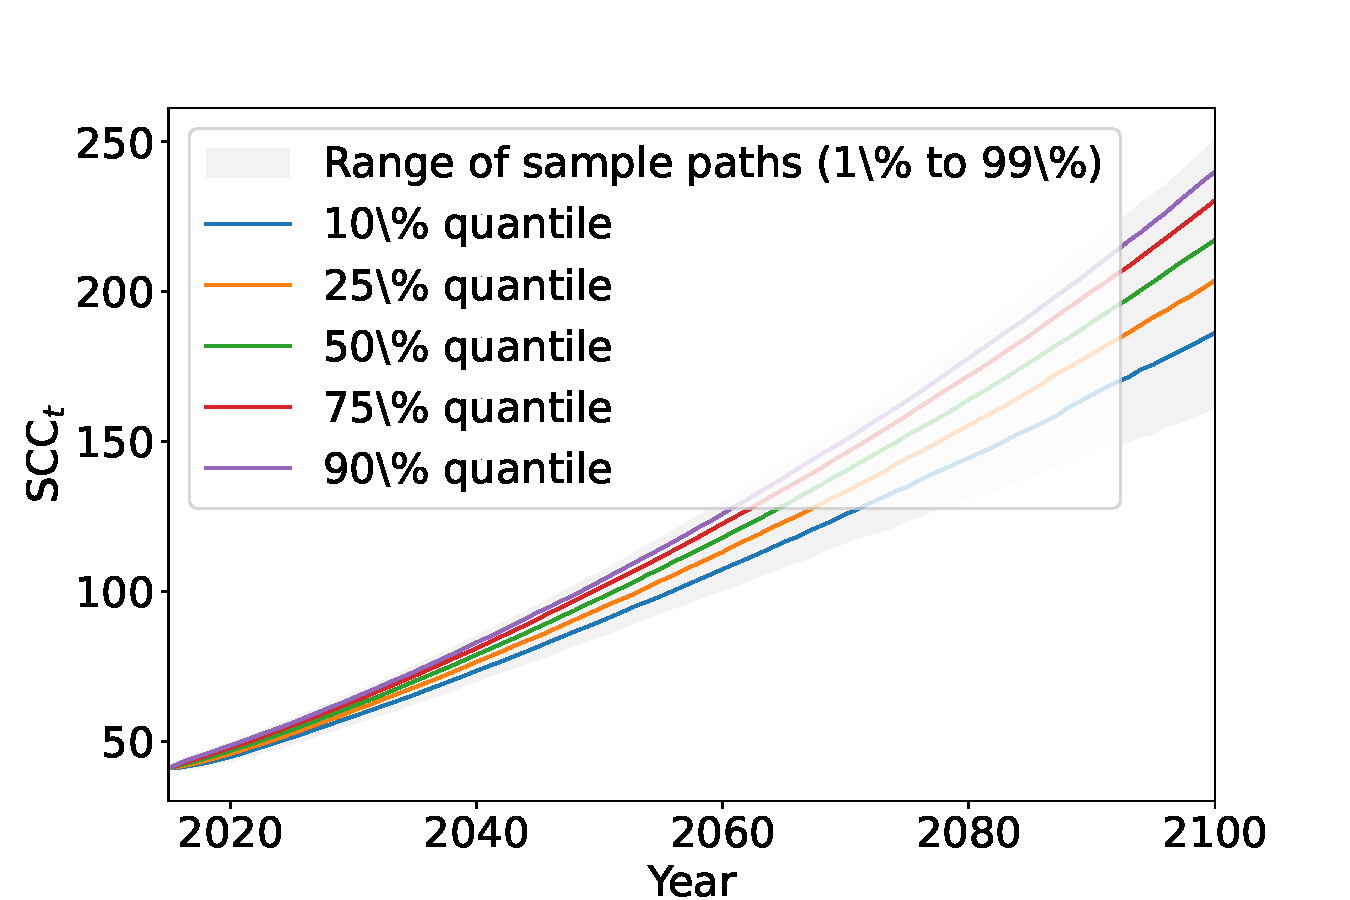
\includegraphics[width=0.44\textwidth]{uq/learn_trunc/benchmark/distribution_2015-2100_scc.pdf}
\end{figure}
{\small Model with no learning (left) and learning (right); SCC behaves like a random variable, as Temperature and ECS are stochastic (our results confirm~\cite{Cai_Lontzek_2019}).}
\end{frame}

% --- Global sensitivity analysis: 3 quantities ---
\begin{frame}{Global Sensitivity Analysis: 3 Quantities}
\small
\begin{itemize}\itemsep3pt
    \item \textbf{\emphc{How are quantitative results of IAMs sensitive to a specific parameterization}}? A \key{importance ranking} informs the researcher on which parts to focus when calibrating or extending a model, or the policymaker on which parameters need further scrutiny.
    \item ``One-at-a-time'' approaches tend to be unstructured and are only \textbf{local}: highly dependent on the chosen parameter values. We aim at determining which input parameters (or combinations) contribute the most to the uncertainty of the QoI, globally.
	\item Measures we use:
	\begin{itemize}
	    \item \keyc{\textbf{Sobol' index}: prioritization of the uncertain parameters based on the outcome variance explained}.
        \item \keyc{\textbf{Shapley value}: identifies how much model variance can be attributed to the uncertainty in input parameters}.
        \item \keyc{\textbf{Univariate effect}: shows how each parameter affects the outcomes}.
	\end{itemize}
\end{itemize}
$\rightarrow$ All three are computed on a cheap-to-evaluate \textbf{surrogate model} based on Gaussian Processes~\citep{scheideggerbilinois_2019}, e.g., SCC($\theta_1, \theta_2,...,\theta_N$).
\end{frame}

% --- Univariate effect ---
\begin{frame}{Univariate Effect (UE)}
\small
\begin{itemize}\itemsep4pt
 \item UE: measures the non-linear relationship between the target QoI and an uncertain input parameter.
    \item UE is the conditional expectation, integrating over the other uncertain parameters $\theta_{-i}$, of the QoI as a function of an input parameter $\theta_{i}$ fixed at an arbitrary value $t$:\footnote{In the source figures the fixed value is denoted $\vartheta_i$; we reserve $\vartheta$ for policy parameters throughout this lecture.}
\begin{align*}
  \mathcal{M}^{ 1 }_{i}\left( t \right) =
  \mathbb{E}_{\theta_{-i}}\left[ Y \mid \theta_{i}=t  \right].
\end{align*}
\end{itemize}
\vspace{0.3em}
$\rightarrow$ Sobol' indices do not include information about the direction in which a parameter affects the quantities of interest.

$\rightarrow$ Univariate effects help to find regions of high and low sensitivity, and can be interpreted as a robust direction of change under parameter uncertainty.
\end{frame}

% --- Univariate effects figure ---
\begin{frame}
\frametitle{Univariate Effects on the SCC in 2020 (Learning Model)}
\begin{figure}
    \centering
    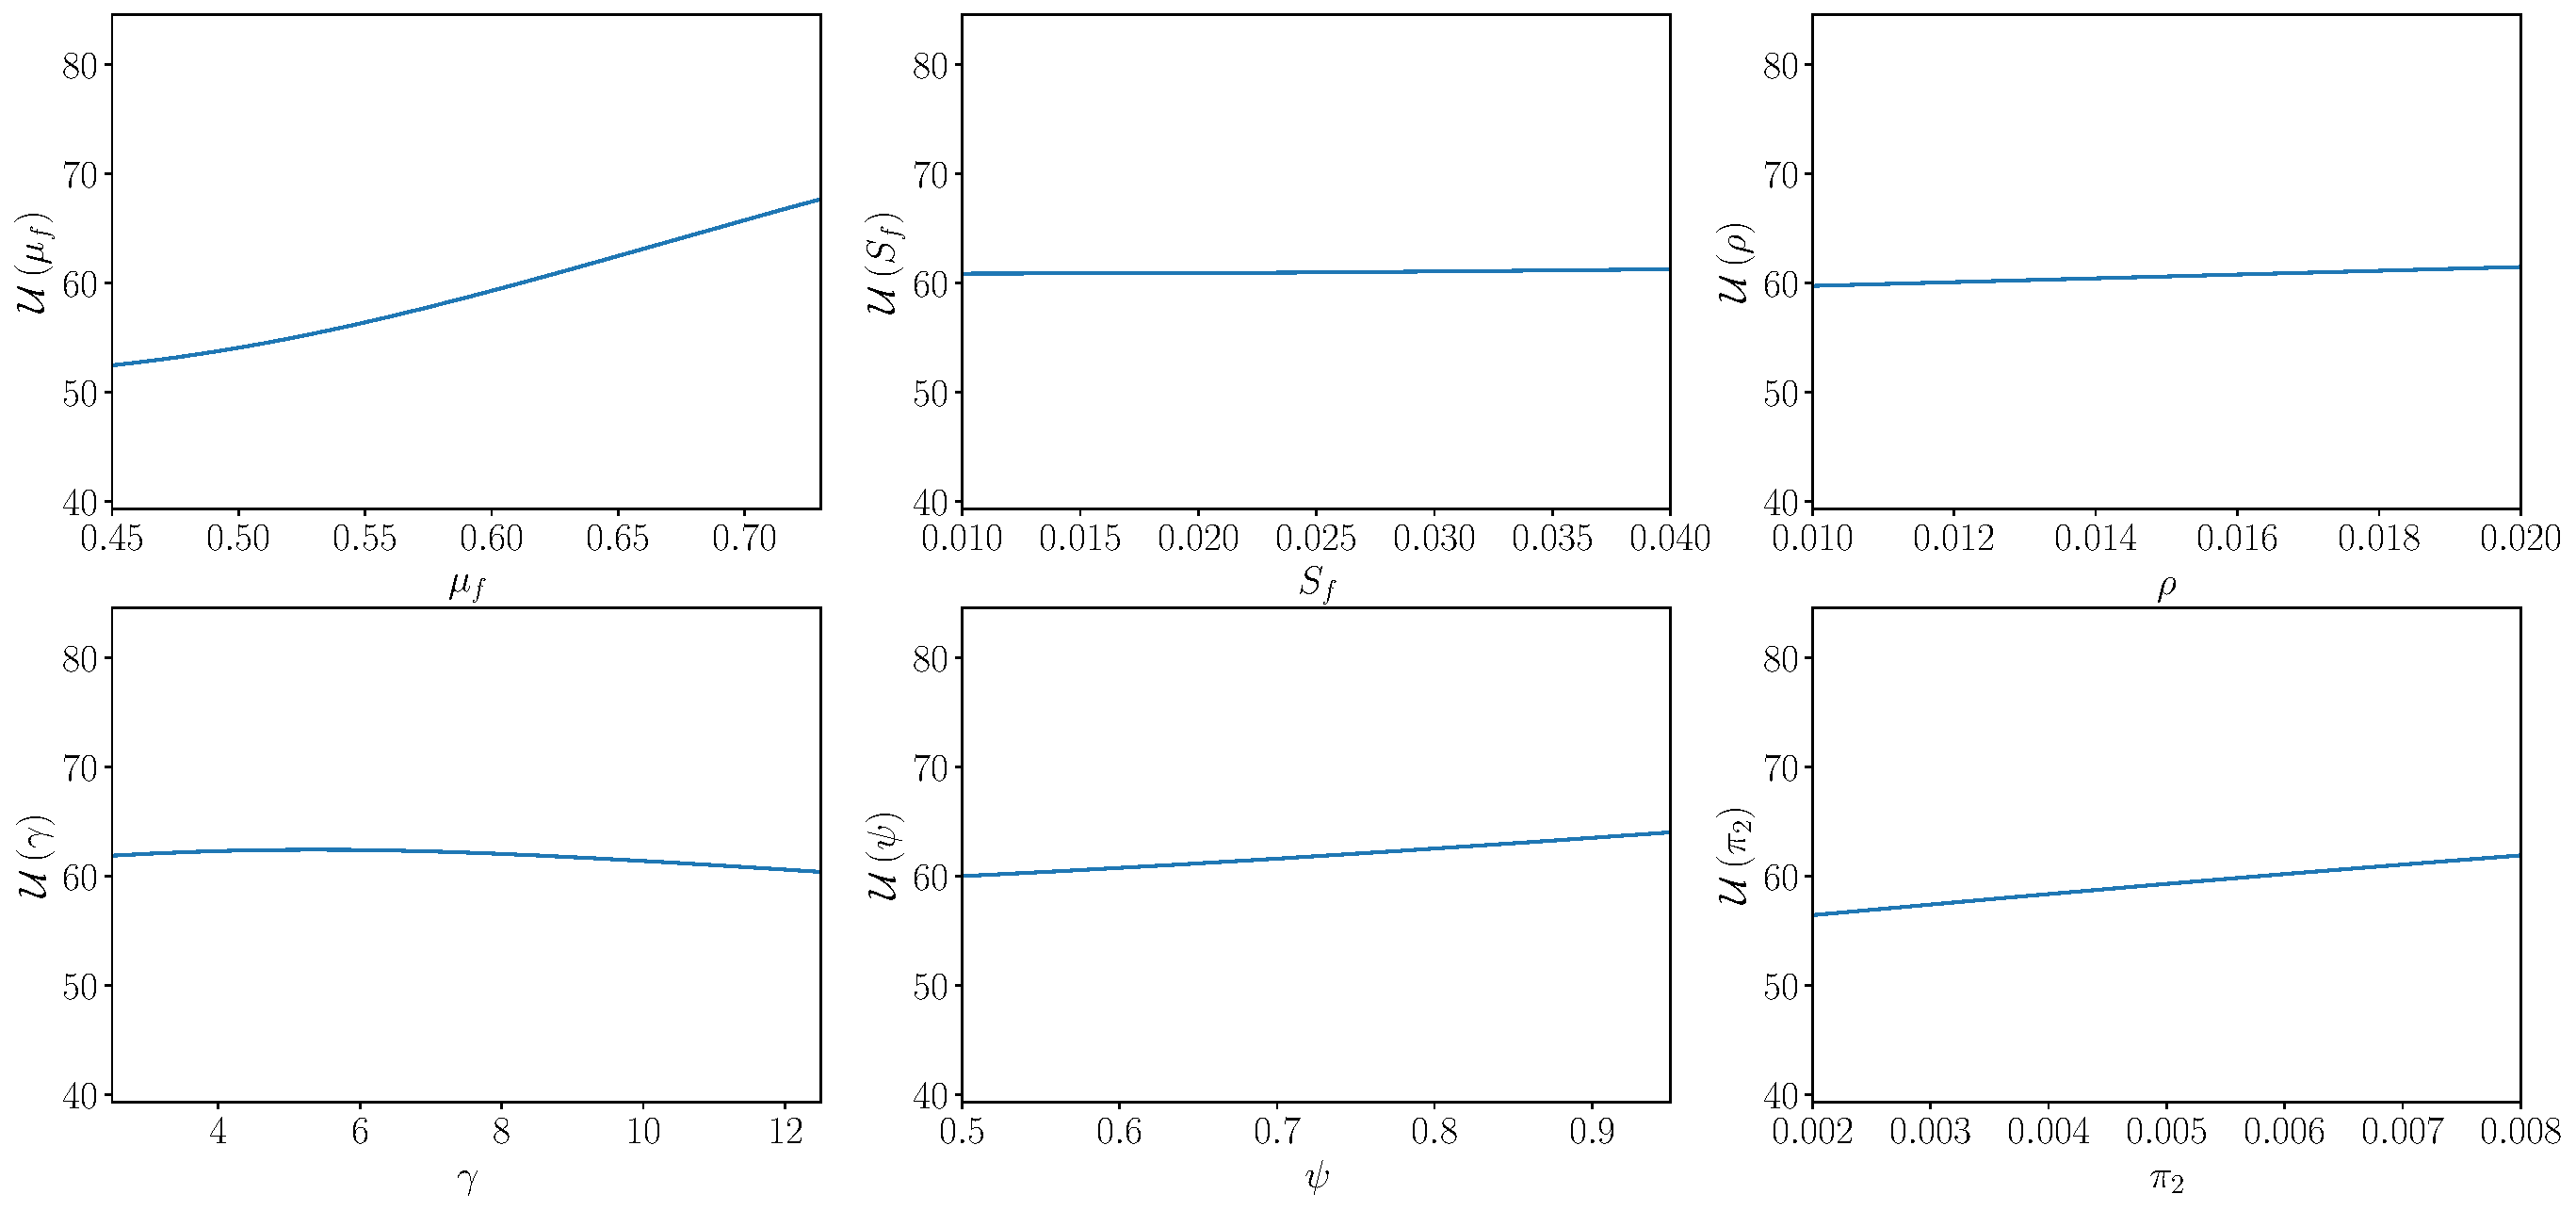
\includegraphics[width=0.92\textwidth]{uq/Learning_upd/uni_pred_E_scc2020_panel.pdf}
\end{figure}
\end{frame}

% --- Sobol' indices ---
\begin{frame}{Sobol' Indices}
\small
\begin{itemize}\itemsep3pt
    \item Consider a generic model $\mathcal{M}\left( \cdot \right)$ with $N$ uncertain input parameters $\theta$ and output $y$ summarizing the QoI (e.g., SCC):
    \begin{align*}
      \theta \in \mathcal{D}_{\theta} \subset \mathbb{R}^{N} \mapsto y =
      \mathcal{M}\left( \theta_{1}, \theta_{2},\cdots,\theta_{N} \right)
      \in \mathbb{R}^{Q}.
    \end{align*}
    \item The first-order Sobol' indices are defined as:\footnote{For simplicity, we assume $Q=1$.}
    \begin{align*}
    S_{i} \equiv \frac{\mathrm{Var}_{\theta_{i}}\left[ \mathbb{E}_{\Theta \setminus \theta_{i}}\left[ y \mid \theta_{i} \right] \right]}{\mathrm{Var}_{\Theta}\left[ y \right]}
    \end{align*}
    \item The numerator measures the first-order effect of $\theta_{i}$ on the model output $y$; normalizing by the total model variance $\mathrm{Var}_{\Theta}\left[ y \right]$ scales the index to $[0, 1]$.
    \item \textbf{Screening interpretation:} the first-order Sobol' index indicates by what percentage the total variance would be reduced, should the parameter $\theta_i$ be perfectly known and set to a fixed value. If it is small (in practice $< 1\%$), $\theta_i$ can be set to a deterministic value without changing the distribution of the QoI.
\end{itemize}
\end{frame}

% --- Importance of parameters ---
\begin{frame}
\frametitle{Importance of Parameters for SCC in 2020}
\begin{figure}
    \centering
        
\includegraphics[width=0.46\textwidth]{uq/nolearn_uq/shapley_S1st_GP_E_scc2020.pdf}
    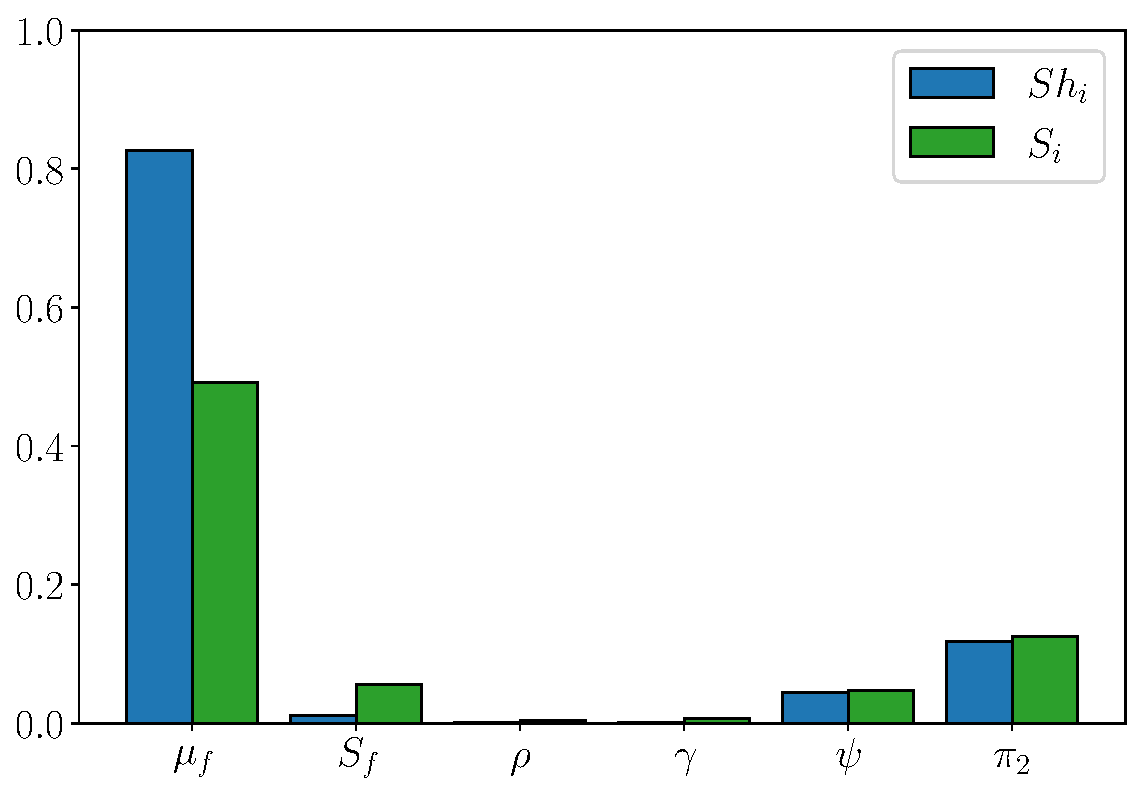
\includegraphics[width=0.46\textwidth]{uq/Learning_upd/shapley_S1st_GP_E_scc2020.pdf}
\end{figure}
UQ results (Shapley values and first-order Sobol' indices) for the model without learning (left) and with learning (right) in 2020.
\end{frame}

% --- UQ takeaways ---
\begin{frame}{UQ Takeaways: What Drives SCC Uncertainty}
\begin{itemize}\itemsep6pt
	\item Uncertainty in SCC is mainly driven by parametric uncertainty in the ECS and the damage function.
 	\item Overall, highly nuanced results.
    \item The quantify operator ran entirely in post-processing: the equilibrium was solved exactly once.
    \item \textbf{Some open-source codes here}:
    \begin{itemize}
        \item \url{https://github.com/ClimateChangeEcon/Climate_in_Climate_Economics}
        \item \url{https://github.com/sischei/DeepEquilibriumNets}
    \end{itemize}
\end{itemize}
\end{frame}


% ============================================================================
% PART V: SYNTHESIS
% ============================================================================

% --- Section divider ---
\begin{frame}{}
\vfill
\begin{center}
{\Huge \textcolor{uzhblue}{\textbf{Part V}}}\\[12pt]
{\LARGE Synthesis: One Surrogate, Three Questions}
\end{center}
\vfill
\end{frame}

% --- Synthesis table ---
\begin{frame}{One Surrogate, Three Questions}
\scriptsize
\begin{center}
\begin{tabular}{p{0.13\textwidth}p{0.24\textwidth}p{0.25\textwidth}p{0.24\textwidth}}
\toprule
 & \textbf{Lecture 2: SMM} & \textbf{Part III: Design} & \textbf{Part IV: Quantify} \\
\midrule
Model & Brock--Mirman & stochastic OLG IAM with tipping risk & stochastic IAM with Bayesian learning about the equilibrium climate sensitivity (ECS) \\
Surrogate inputs & state plus estimation pseudo-states & OLG IAM state plus 16 policy pseudo-states & climate-economy states plus uncertain $\bm{\theta}$ (9+N states) \\
QoI & a few moments & 40 cohort welfares & $\mathrm{SCC}(\bm{\theta})$ \\
Second surrogate & none needed & GP $\times 40$ with BAL & GP + Bayesian active learning \\
Operator & $\argmin$ & constrained $\argmax$ & global sensitivity analysis (UE, Sobol', Shapley) \\
Output & parameter estimate & Pareto-improving tax & importance ranking of parameters \\
Headline & the criterion's shape carries the lesson & 0.42\% aggregate gain, no generation loses & ECS and damage-function uncertainty drive the SCC \\
\bottomrule
\end{tabular}
\end{center}
\end{frame}

% --- Practical guidance ---
\begin{frame}{Practical Guidance}
\small
\begin{itemize}\itemsep6pt
\item \textbf{Train once, then simulate for free.} Surrogate 1 costs about 4h from scratch on a laptop, a few minutes warm-started; once trained, the solution allows us to simulate data essentially for free.
\item \textbf{When the second surrogate pays off.} Whenever a single QoI point is expensive: expected welfare needs 10{,}000 Monte Carlo paths per policy $\vartheta$; the GP + BAL layer reduces this to 500 simulations total (450 Latin hypercube + 50 actively learned), at LOO error $\approx 10^{-4}$.
\item \textbf{A generic blueprint.} A universal framework for \textbf{almost any} stochastic heterogeneous-agent model: it allows researchers to both \keyc{solve global equilibria} and derive \keyc{constrained-optimal policies} in settings previously deemed intractable.
\item \textbf{Production-scale reference.} Chen, Didisheim \& Scheidegger (2026, \emph{J.\ Financial Economics}): exactly this surrogate logic at scale, applied to finance.
\end{itemize}
\end{frame}

% --- Extensions and open questions ---
\begin{frame}{Extensions and Open Questions}
\small
\textbf{Extensions on the authors' agenda:}
\begin{itemize}\itemsep2pt
\item Analyze richer, non-linear tax functions, solve for the optimal tax, and construct the Pareto frontier.
\item Optimal transfers in a ``quadratic'' (parametrized) tax model.
\item Based on high-dimensional model representation~\citep{eftekhari_2022}, determine the dominant terms that are driving the results.
\item Add multiple global regions to the model to study the distributional effects of climate change.
\end{itemize}
\vspace{0.5em}
\textbf{Open questions (bridges between Part III and Part IV):}
\begin{itemize}\itemsep2pt
\item Apply the \emphc{quantify} operator to the \emphc{design} output: how sensitive is $\vartheta^*(\bm{\theta})$ to the structural parameters?
\item Propagate Lecture 2-style estimation uncertainty in $\hat{\bm{\theta}}$ into the SCC.
\end{itemize}
\end{frame}

% --- Conclusion ---
\begin{frame}{Conclusion}
    \begin{columns}
        \begin{column}{0.62\textwidth}
            \footnotesize
            \begin{itemize}
                \setlength{\itemsep}{0.7em}
                \item \textbf{One pipeline, three operators:} \\
                A scalable ML framework (\keyc{DEQN + GP + post-processing}) supports \emphc{estimate} (Lecture 2: SMM), \emphc{design}, and \emphc{quantify} on the same trained surrogate.
                \item \textbf{Design (Part III):} \\
                Simple linear tax + optimal transfers $\rightarrow$ \textbf{Pareto improvement}, with a \textbf{0.42\%} aggregate welfare gain; added complexity yields only marginal gains (to \textbf{0.45\%}): simple, implementable rules capture the vast majority of benefits.
                \item \textbf{Quantify (Part IV):} \\
                Uncertainty in the SCC is mainly driven by parametric uncertainty in the ECS and the damage function.
                \item \emphc{Solve once, ask many questions.}
            \end{itemize}
        \end{column}
        \begin{column}{0.36\textwidth}
            \centering
            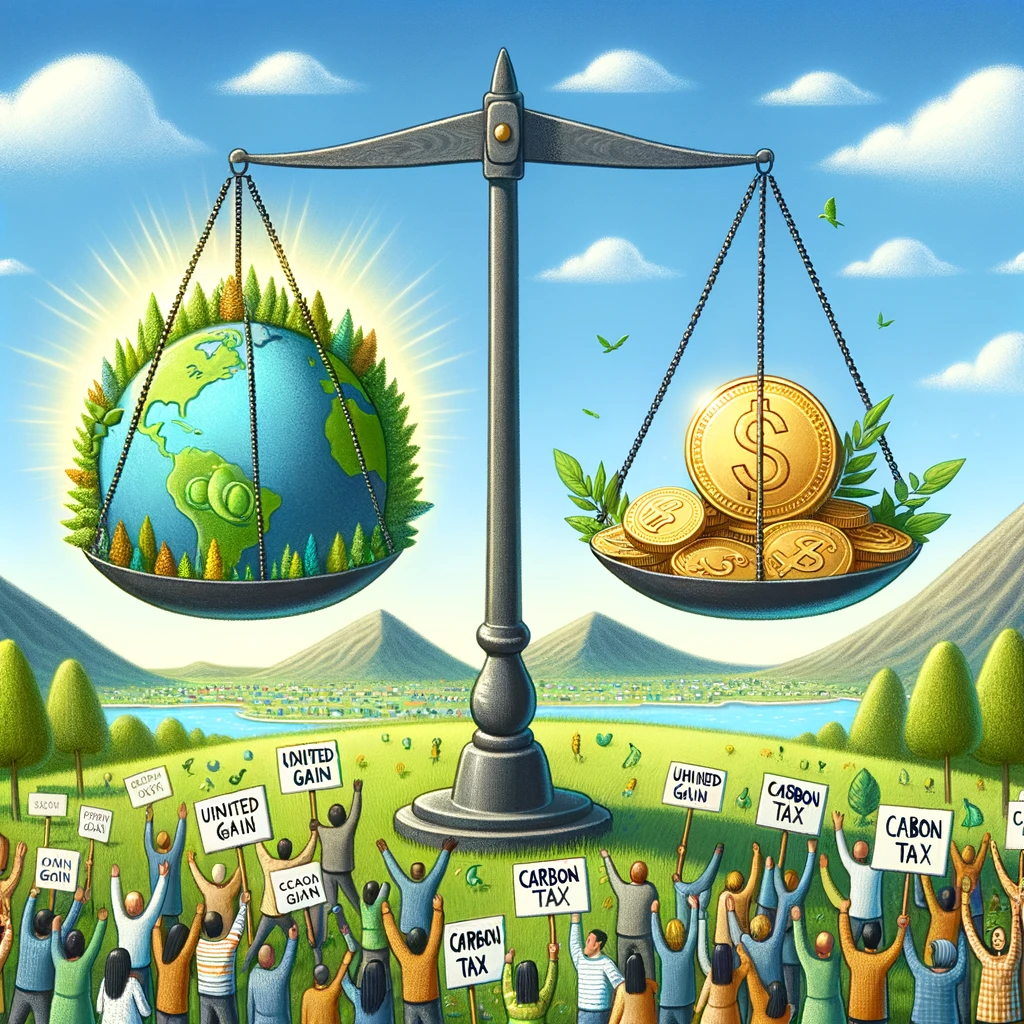
\includegraphics[width=0.9\linewidth]{tax/summary_happy.png}
        \end{column}
    \end{columns}
\end{frame}


% ============================================================================
% CLOSING
% ============================================================================

% --- Bridge frame ---
\begin{frame}{The Course in One Slide}
\footnotesize
\textbf{The three-lecture arc.}
\begin{enumerate}\itemsep2pt
    \item \textbf{Lecture 1 --- Solve.} Deep Equilibrium Nets: global solutions of dynamic (stochastic) models from equilibrium residuals, from Brock--Mirman to the IRBC model.
    \item \textbf{Lecture 2 --- Map and apply.} Deep surrogates, GPs, Bayesian active learning, structural estimation; the DICE/CDICE climate--economy model solved with DEQNs.
    \item \textbf{Lecture 3 --- Decide.} The same machinery answers policy questions: constrained optimal carbon taxes (design) and the uncertainty of the SCC (quantify).
\end{enumerate}

\vspace{0.2em}
\textbf{Where to go next.}
\begin{itemize}\itemsep2pt
    \item Tax replication code: {\scriptsize \url{https://github.com/sischei/JPE_Macro_Using_ML_to_compute_constrained_optimal_carbon_tax_rules}}
    \item CDICE production code: {\scriptsize \url{https://github.com/ClimateChangeEcon/Climate_in_Climate_Economics}}
    \item Textbook-style treatment, notes, and code: {\scriptsize \url{https://github.com/sischei/Deep_Learning_for_Solving_And_Estimating_Dynamic_Economic_Models}}
\end{itemize}

\vspace{0.2em}
{\scriptsize \textbf{References.} K\"ubler, Scheidegger \& Surbek (2026, \emph{JPE: Macro}); Friedl, K\"ubler, Scheidegger \& Usui (2023); Azinovic, Gaegauf \& Scheidegger (2022, \emph{IER}); Folini, Friedl, K\"ubler \& Scheidegger (2025, \emph{REStud}).}
\end{frame}

% --- Questions ---
\begin{frame}{}
\begin{columns}[c]
\column{0.45\textwidth}
\begin{center}
{\Huge \textcolor{uzhblue}{\textbf{Questions?}}}

\vspace{1.0cm}
{\large Simon Scheidegger}\\[4pt]
{\small HEC Lausanne $\cdot$ Grantham Research Institute, LSE}\\[4pt]
\url{https://sischei.github.io}

\vspace{0.6cm}
{\small Materials:~~\url{https://github.com/sischei/cemracs2026_DEQN}}
\end{center}

\column{0.45\textwidth}
\begin{center}
\textbf{Next up:}\\[6pt]
{\large Practical session: hands-on\\[2pt]
surrogates, DICE, and UQ}\\[12pt]
{\small Notebooks: \texttt{lectures/lecture\_2/code/}\\[2pt]
Tax replication code: \texttt{lectures/lecture\_3/code/}}
\end{center}
\end{columns}
\end{frame}


% ============================================================================
% APPENDIX
% ============================================================================
\appendix

% --- Sampling domain ---
\begin{frame}[fragile]{Appendix: Sampling Domain}
\begin{table}[ht!]
\centering
\small
\begin{tabular}{lllll}
\toprule
Model & Planner Target & Parameter & $\underline{\vartheta_i}$ & $\bar{\vartheta_i}$ \\
\midrule
Linear in E & Max. Welfare & $\vartheta_0$     & -2.0   & 2.0   \\
            & Max. Welfare & $\vartheta_E$     & -2.0   & 2.0  \\
           & Max. Welfare & $\tau$         & 0.0  & 1.5  \\
            \midrule
Linear in E + Transfers & Pareto & $\vartheta_0$ & -0.5 & 0.1 \\
                        & Pareto & $\vartheta_E$ & 0.0    & 0.5 \\
                        & Pareto & $\tau$         & 0.0  & 0.8  \\
\midrule
Full linear + Transfers & Pareto & $\vartheta_0$     & -1.0   & 0.5 \\
                        & Pareto & $\vartheta_E$     & -0.5 & 1.0   \\
                        & Pareto & $\vartheta_\kappa$ & -0.6 & 0.6 \\
                        & Pareto & $\vartheta_{TP}$   & -1.0   & 1.0   \\
                        & Pareto & $\tau$         & 0.0  & 0.8  \\
\bottomrule
\end{tabular}
\caption{Parameter bounds across models and objectives.}
\label{tab:param_bounds_main}
\end{table}
\end{frame}

% --- Quantifying uncertainty about ECS ---
\begin{frame}
\frametitle{Appendix: Quantifying uncertainty about ECS}
\small
\begin{itemize}
\item Temperature equation:
\begin{align}
T_{\mathrm{AT},t+1} = \left(1-\varphi_{21} - \varphi_1\frac{F_{\mathrm{2xco2}}}{\stoch{\Delta T_{\mathrm{AT},\times 2}}}\right)T_{\mathrm{AT},t}+\varphi_{21}T_{\mathrm{OC},t}+\\
\varphi_1 \left(F_{\mathrm{2xco2}} \log_2 \left(\frac{M_{\mathrm{AT},t}}{M_{\mathrm{AT}}^\ast} \right)+F_{\mathrm{EX},t} \right)
\end{align}
    \item Follow \cite{roe2007climate} to make ECS stochastic.
    \item $\mathrm{ECS}=\frac{\lambda_0}{1-f} F_{\mathrm{2XCO2}}$, with climate feedback parameter $ f \sim  \mathcal{N}\left(\mu_{f}, S_f \right) $.
\item  This is controversial, see \cite{zaliapin2010another} and \cite{roe2011comment} and \cite{zaliapin2011reply}.
\end{itemize}
\end{frame}

% --- Bayesian learning mechanics ---
\begin{frame}
\frametitle{Appendix: Bayesian learning mechanics}
\small
\begin{itemize}
    \item Temperature evolves as:
\resizebox{0.75\linewidth}{!}{
  \begin{minipage}{\linewidth}
      \begin{align*}
&T_{\mathrm{AT},t+1} = \left(\varphi_1\frac{F_{\mathrm{2xco2}}}{\Delta T_{\mathrm{AT},\times 2}^{0}} \stoch{\tilde{f}_{t+1}} + 1-\varphi_{21} - \varphi_{1}\frac{F_{\mathrm{2xco2}}}{\Delta T_{\mathrm{AT},\times 2}^{0}} \right)T_{\mathrm{AT},t}\\
&+\varphi_{21}T_{\mathrm{OC},t}+\varphi_1 \left(F_{\mathrm{2xco2}} \log_2 \left(\frac{M_{\mathrm{AT},t}}{M_{\mathrm{AT}}^\ast} \right)+F_{\mathrm{EX},t} \right) + \stoch{\tilde{\epsilon}_{T, t+1}}
\end{align*}
\end{minipage}}

where $\stoch{\tilde{f}_{t+1}} \sim \mathcal{N}\left( \mu_{f,t}, S_{f, t}, \underline{f}, \overline{f} \right)$: uncertain climate sensitivity,  $\stoch{\tilde \epsilon_{T, t+1}}$: shock to the temperature.
    \item The agent observes a realisation of the shocks in climate sensitivity and temperature at the beginning of the period $t$ before the decisions are made.
    \item Under Gaussian assumption analytic formulas for updating:
\resizebox{0.75\linewidth}{!}{
  \begin{minipage}{\linewidth}
    \begin{align*}
& \mu_{f,t+1} = \frac{
 S_{\epsilon_{T}} \mu_{f,t} +  \varphi_{1C} T_{\mathrm{AT}, t}  \left( \varphi_{1C} T_{\mathrm{AT}, t} \tilde{f}_{t+1} + \tilde{\epsilon}_{T,t+1}  \right) S_{f, t}}{S_{\epsilon_{T}} + \left(\varphi_{1C} T_{\mathrm{AT}, t} \right)^2 S_{f, t} }\\
 & S_{f, t+1} = \frac{S_{\epsilon_{T}} S_{f, t}}{S_{\epsilon_{T}} + \left( \varphi_{1C} T_{\mathrm{AT}, t} \right)^{2} S_{f, t}}
\end{align*}
\end{minipage}}
\end{itemize}
\end{frame}

% --- Tail learning ---
\begin{frame}[fragile]{Appendix: Tail learning}
\begin{figure}[t!]
\centering
\begin{subfigure}[t]{0.36\linewidth}
    \centering
    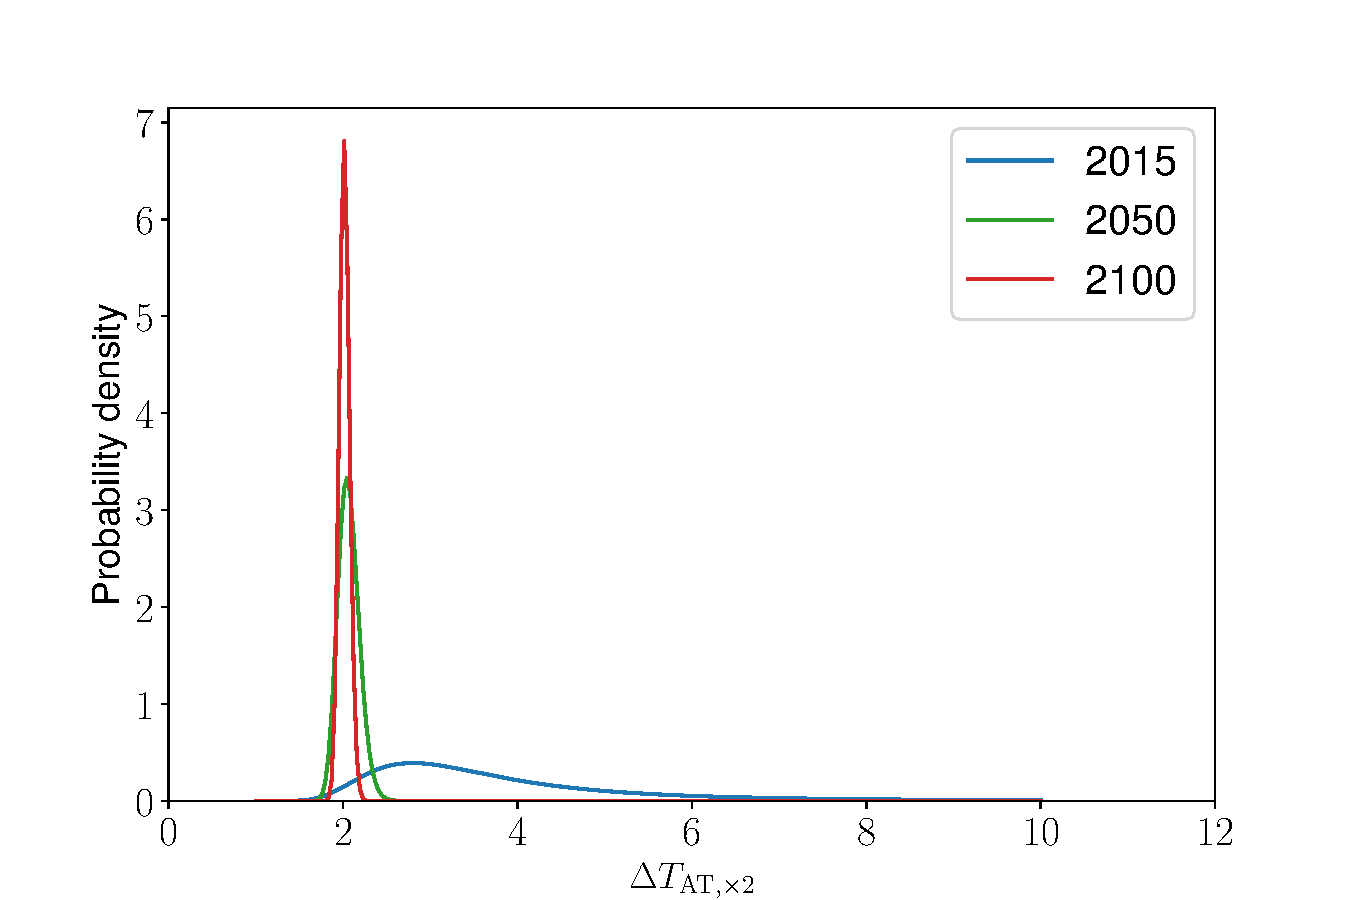
\includegraphics[width=1.0\linewidth]{uq/tail_learning/posterior_ECS_years_truef0.4.pdf}
    \caption{$\Delta T^{\ast}_{\mathrm{AT}, \times 2}=2.0$}
    \label{fig:posterior_distribution_ECS2.0}
\end{subfigure}
\hfill
\begin{subfigure}[t]{0.36\linewidth}
    \centering
    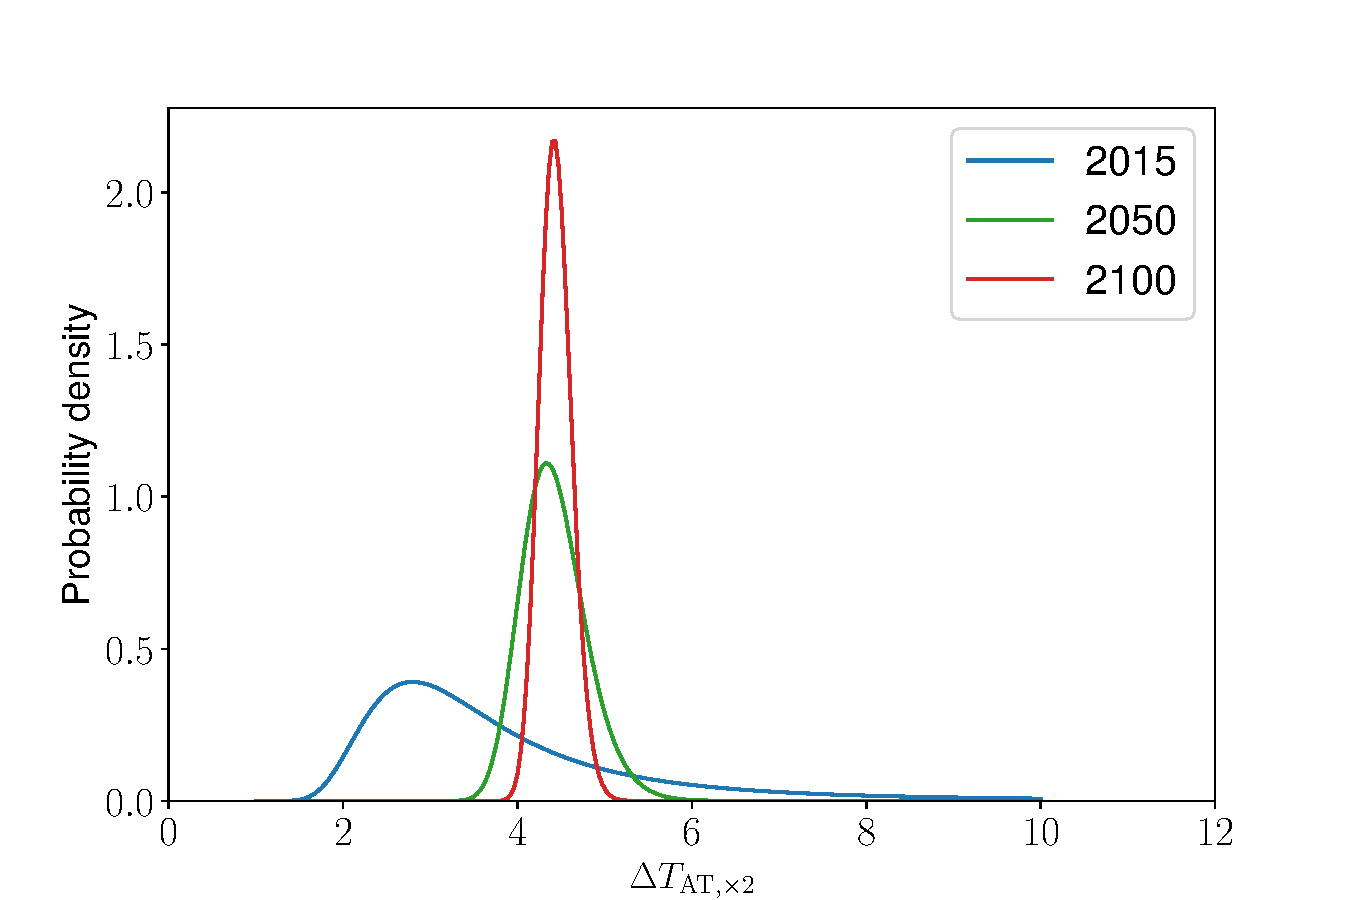
\includegraphics[width=1.0\linewidth]{uq/tail_learning/posterior_ECS_years_truef0.73.pdf}
    \caption{$\Delta T^{\ast}_{\mathrm{AT}, \times 2}=4.5$}
    \label{fig:posterior_distribution_ECS4.5}
\end{subfigure}
\caption{The posterior probability density function of $\Delta T_{\mathrm{AT}, \times 2}$ is shown when the true equilibrium sensitivity $\Delta T^{\ast}_{\mathrm{AT}, \times 2}$ is set to 2.0 and 4.5, respectively.}
\label{fig:posterior_density_ECS}
\end{figure}
\begin{scriptsize}
\begin{itemize}
    \item Social planner learns the upper tail of the prior distribution very quickly (less than a decade for 99\% percentile; ECS $< 3.42$).
    \item In the case where the ECS is set to 4.5, that is, relatively high, learning slows as the Bayes rule requires more observations to move the mean estimate from the prior ECS to the true high value.
\end{itemize}
\end{scriptsize}
\end{frame}

% --- References ---
\begin{frame}[allowframebreaks]{References}
  \bibliography{refs}
  \bibliographystyle{apalike}
\end{frame}

\end{document}
